\documentclass[aspectratio=169]{beamer}

\usetheme{Madrid}

\definecolor{NavyTIPE}{RGB}{0,42,92}
\definecolor{CyanTIPE}{RGB}{0,160,200}
\definecolor{LightCyan}{RGB}{220,244,252}

\setbeamercolor{palette primary}   {bg=NavyTIPE, fg=white}
\setbeamercolor{palette secondary} {bg=CyanTIPE, fg=white}
\setbeamercolor{palette tertiary}  {bg=NavyTIPE, fg=white}
\setbeamercolor{palette quaternary}{bg=NavyTIPE, fg=white}
\setbeamercolor{structure}{fg=NavyTIPE}
\setbeamercolor{title}{fg=white, bg=NavyTIPE}
\setbeamercolor{frametitle}{fg=white, bg=NavyTIPE}
\setbeamercolor{block title}{bg=NavyTIPE, fg=white}
\setbeamercolor{block body}{bg=LightCyan, fg=black}
\setbeamercolor{block title alerted}{bg=CyanTIPE, fg=white}
\setbeamercolor{block body alerted}{bg=LightCyan, fg=black}
\setbeamercolor{alerted text}{fg=CyanTIPE}

\setbeamertemplate{bibliography item}{}

\usepackage[utf8]{inputenc}
\usepackage[T1]{fontenc}
\usepackage[french]{babel}
\usepackage{csquotes}

\usepackage{amsmath, amssymb}
\usepackage{graphicx}
\graphicspath{{imageIllustration/}}
\usepackage{hyperref}
\usepackage{array}
\usepackage{colortbl}

\usepackage{tikz}
\usetikzlibrary{arrows.meta, decorations.pathmorphing, decorations.markings,
decorations.pathreplacing, patterns, calc, positioning, shapes.geometric}

\usepackage{listings}
\definecolor{codegreen}{rgb}{0,0.6,0}
\definecolor{codegray}{rgb}{0.5,0.5,0.5}
\definecolor{codepurple}{rgb}{0.58,0,0.82}
\definecolor{backcolour}{rgb}{0.95,0.95,0.92}
\lstdefinestyle{mystyle}{
  backgroundcolor=\color{backcolour},
  commentstyle=\color{codegreen},
  keywordstyle=\color{NavyTIPE},
  numberstyle=\tiny\color{codegray},
  stringstyle=\color{codepurple},
  basicstyle=\ttfamily\tiny,
  breakatwhitespace=false,
  breaklines=true,
  captionpos=b,
  keepspaces=true,
  numbers=left,
  numbersep=5pt,
  showspaces=false,
  showstringspaces=false,
  showtabs=false,
  tabsize=2,
  literate={é}{{\'e}}1 {è}{{\`e}}1 {à}{{\`a}}1 {ç}{{\c{c}}}1 {œ}{{\oe}}1 {ù}{{\`u}}1 {À}{{\`A}}1 {É}{{\'E}}1 {Ê}{{\^E}}1 {ê}{{\^e}}1 {î}{{\^i}}1 {ô}{{\^o}}1 {û}{{\^u}}1 {â}{{\^a}}1 {ï}{{\"i}}1 {ë}{{\"e}}1 {°}{{$^\circ$}}1
}
\lstset{style=mystyle}

\title[TIPE - Efficacité Propulsive]{%
  Influence de la flexibilité d'une hélice de drone\\
sur l'efficacité de propulsion}
\subtitle{Bilan de la 1\texorpdfstring{\textsuperscript{ère}}{ère} année, avancées des vacances, et objectifs}
\author{Merlin Claret}
\institute{PT* — Lycée La Martinière Monplaisir, Lyon}
\date{Rentrée Septembre 2026}

\begin{document}

\begin{frame}[plain]
  \titlepage
\end{frame}

\begin{frame}{Plan de la présentation}
  \tableofcontents
\end{frame}

% =========================================================================
\section{Le Sujet}
% =========================================================================

\begin{frame}{Contexte et problématique}
  \begin{columns}
    \column{0.66\textwidth}
    \textbf{Problématique du TIPE :}
    \begin{block}{}
      \small
      \textit{Comment quantifier l'influence de la rigidité d'une hélice sur sa déformation en vol et sur l'efficacité de propulsion ?}
    \end{block}

    \vspace{0.1cm}
    \textbf{Déformation :}
    \begin{itemize}
      \item À haut régime, les efforts aérodynamiques déforment les pales (\alert{flexion et torsion}).
      \item L'incidence locale est modifiée, ce qui impacte le rendement propulsif.
    \end{itemize}

    \vspace{0.1cm}
    \textbf{Démarche :}
    \begin{itemize}
      \item \textbf{Modélisation :} Prédire la déformation et la perte de poussée (Python).
      \item \textbf{Expérimentation :} Comparer sur un banc d'essai deux hélices de 5 pouces :
        \textbf{Nylon} (souple) vs \textbf{Carbone} (rigide).
    \end{itemize}

    \column{0.38\textwidth}
    \centering
    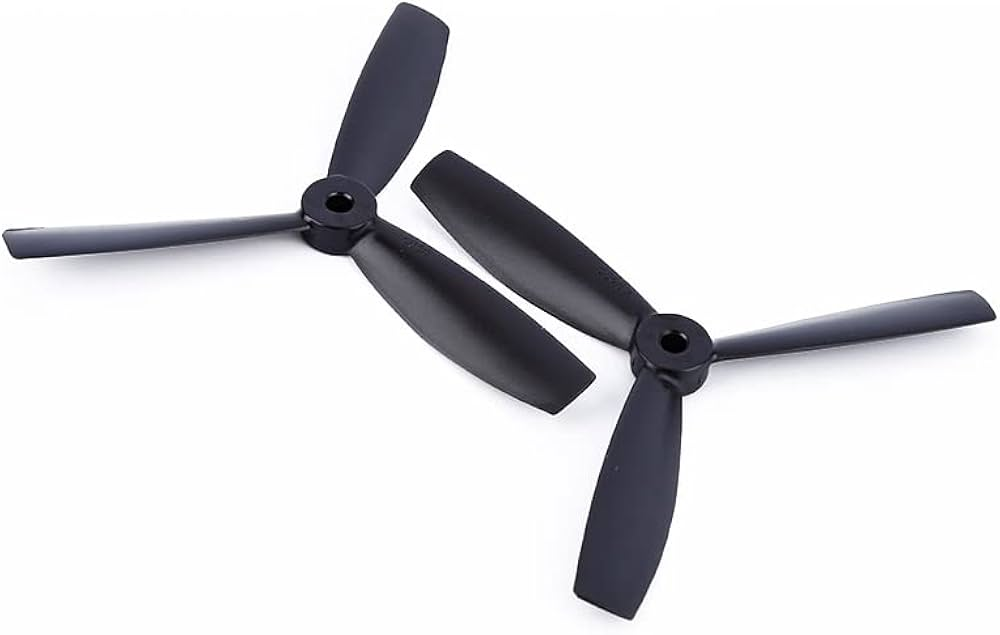
\includegraphics[width=0.65\textwidth,keepaspectratio]{helice5pouce.jpg}
  \end{columns}
\end{frame}

% =========================================================================
\section{Bilan de la 1\texorpdfstring{\textsuperscript{ère}}{ère} année : Ce qui a été fait (et les difficultés)}
% =========================================================================

\begin{frame}{Simulation et limites expérimentales}
  \textbf{Modèle physique couplé (BET + RDM) développé en Python :}
  \begin{itemize}
    \item \textbf{Aérodynamique (BET) :} Discrétisation en éléments de pale.
    \item \textbf{RDM (Poutre en torsion) :} Évaluation de la torsion en fonction des efforts aérodynamiques.
    \item \textbf{Boucle itérative :} Déformation $\implies$ modification de l'incidence $\implies$ perte de poussée.
  \end{itemize}

  \begin{alertblock}{Ordres de grandeur et besoin de précision}
    Pour une hélice de drone 5 pouces, la \textbf{vitesse de rotation maximale} est très élevée : $\approx \textbf{25\,000 à 30\,000\text{ tr/min}}$.\\
    À ce régime, le modèle prédit un écart de poussée $\Delta T \approx 1\text{ N} \ (\sim 100\text{ g})$ entre une hélice souple et une rigide.\\
    $\implies$ Il faut concevoir un banc d'essai avec des frottements $\ll 100\text{ g}$.
  \end{alertblock}
\end{frame}

\begin{frame}{Le premier banc d'essai (Prototype 1) : pas très intelligent}
  \begin{columns}
    \column{0.58\textwidth}
    \textbf{Principe initial (fin de 1\textsuperscript{ère} année) :}
    \begin{itemize}
      \item Guidage linéaire par chariot avec 4 douilles à billes sur des colonnes.
    \end{itemize}

    \vspace{0.2cm}
    \textbf{Pourquoi abandonner ce banc :}
    \begin{itemize}
      \item \textbf{Frottements secs :} beaucoup trop important pour isoler de façon fiable une différence de $100\text{ g}$.
      \item \textbf{Masque :} La platine (et le sol) obstruait le flux d'air de l'hélice.
      \item \textbf{Risque d'arc-boutement :} Poussée trop déportée par rapport au guidage.
    \end{itemize}

    \column{0.42\textwidth}
    \centering
    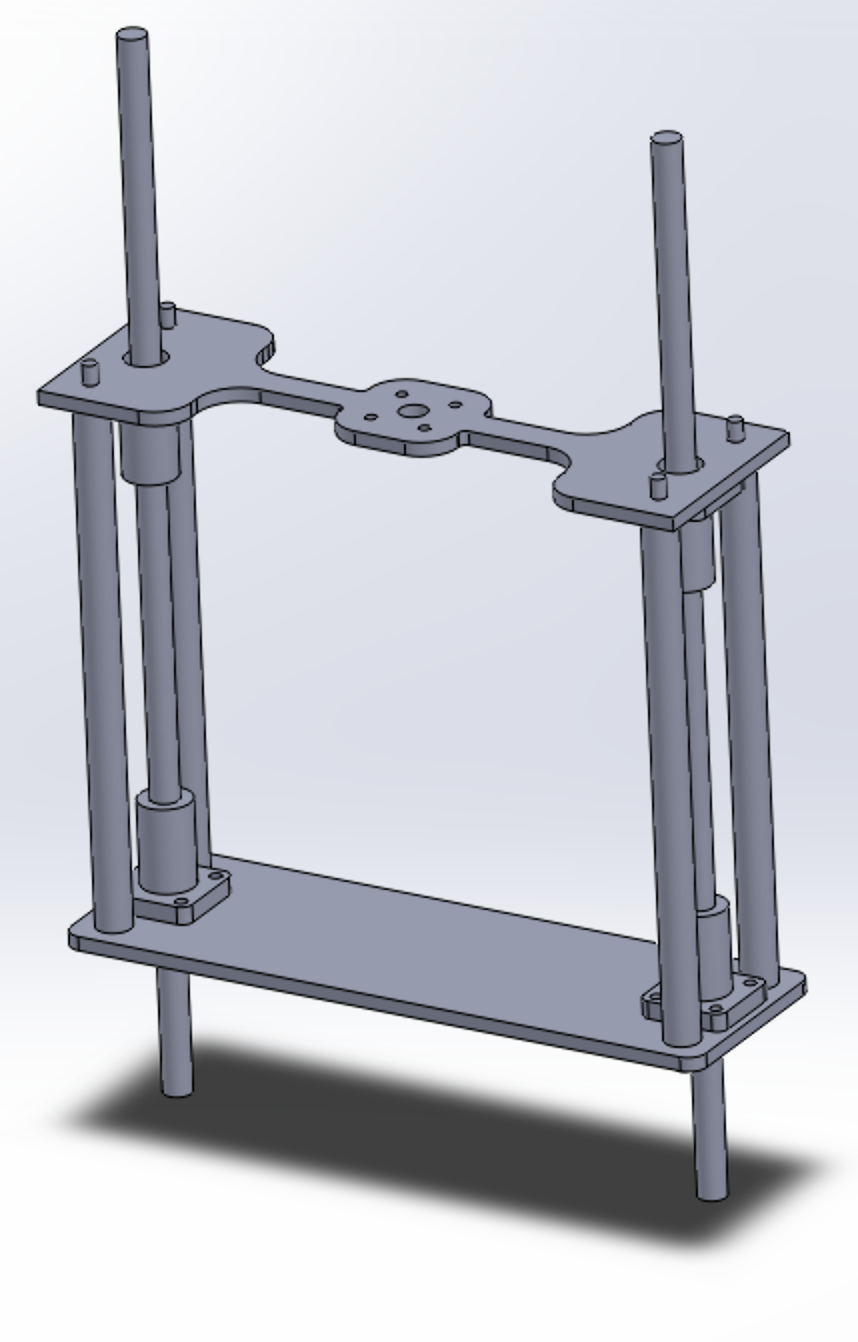
\includegraphics[width=0.95\textwidth,height=0.52\textheight,keepaspectratio]{chariotAssembl.png}
    \par\vspace{2pt}{\scriptsize \textit{Prototype 1 (chariot) abandonné}}
  \end{columns}
\end{frame}

% =========================================================================
\section{Avancées des vacances : Nouvelle architecture}
% =========================================================================

\begin{frame}{Nouvelle Architecture (Été) : Le Banc Pendulaire}
  \begin{columns}
    \column{0.50\textwidth}
    \centering
    \begin{tikzpicture}[scale=0.68, every node/.style={scale=0.75}]
      % Sol
      \fill[pattern=north east lines, pattern color=gray!50] (-0.8, -0.3) rectangle (4.6, 0);
      \draw[thick] (-0.8, 0) -- (4.6, 0);

      % Bâti fixe
      \draw[fill=gray!25, thick] (-0.25, 0) rectangle (0.25, 2.5);
      \node[anchor=east] at (-0.3, 1.25) {\textbf{Bâti fixe}};

      % Pivot
      \draw[fill=NavyTIPE, thick] (0, 2.5) circle (0.25);
      \draw[fill=white] (0, 2.5) circle (0.09);
      \node[anchor=south east, NavyTIPE] at (-0.1, 2.75) {\textbf{Pivot}};

      % Bras vertical (L1 = 140 mm)
      \draw[NavyTIPE, very thick, fill=LightCyan] (-0.12, 2.5) rectangle (0.12, 4.8);
      \draw[<->, thick, NavyTIPE] (-0.45, 2.5) -- (-0.45, 4.8) node[midway, left] {$L_1 = 140\text{ mm}$};

      % Moteur + Hélice
      \draw[fill=gray!80, thick] (-0.35, 4.8) rectangle (0.35, 5.2);
      \node[above right, NavyTIPE] at (0.35, 5.25) {\scriptsize \textbf{Moteur}};
      \draw[line width=1.5pt, gray!50] (0.35, 4.2) -- (0.35, 5.8);

      % Poussée T
      \draw[-{Latex[length=3mm]}, red, line width=2pt] (-2.1, 5.0) -- (-0.35, 5.0);
      \node[below, red] at (-1.25, 4.95) {\scriptsize \textbf{Poussée} $\vec{T}$};

      % Bras horizontal (L2 = 200 mm)
      \draw[NavyTIPE, very thick, fill=LightCyan] (0, 2.38) rectangle (3.6, 2.62);
      \draw[<->, thick, NavyTIPE] (0, 2.9) -- (3.6, 2.9) node[midway, above] {$L_2 = 200\text{ mm}$};

      % Force mesurée
      \draw[very thick] (3.4, 2.38) -- (3.4, 0.8);
      \draw[-{Latex[length=3mm]}, red, line width=2pt] (3.4, 1.8) -- (3.4, 0.5) node[midway, right] {$\vec{F}_{\text{mes}}$};

      % Capteur
      \draw[fill=CyanTIPE!30, thick] (2.7, 0.05) rectangle (4.1, 0.55);
      \node at (3.4, 0.3) {\textbf{Capteur / Balance}};
    \end{tikzpicture}

    \column{0.50\textwidth}
    \textbf{Principe de la nouvelle solution :}
    \begin{itemize}
      \item \textbf{Aérodynamisme optimisé :} Bras pendulaire fin ($20 \times 20\text{ mm}$) dans le sillage du moteur pour ne pas perturber trop le flux d'air.
      \item \textbf{Pivot :} Utilisation de roulements à billes pour minimiser les pertes, pour l'instant pas de roulements.
      \item \textbf{Principe pendule :} Permet d'amplifier l'effort mesuré avec la balance grâce au rapport des bras de levier $L_1$ et $L_2$.
    \end{itemize}
  \end{columns}
\end{frame}

\begin{frame}{Étude statique du banc pendulaire}
  \centering
  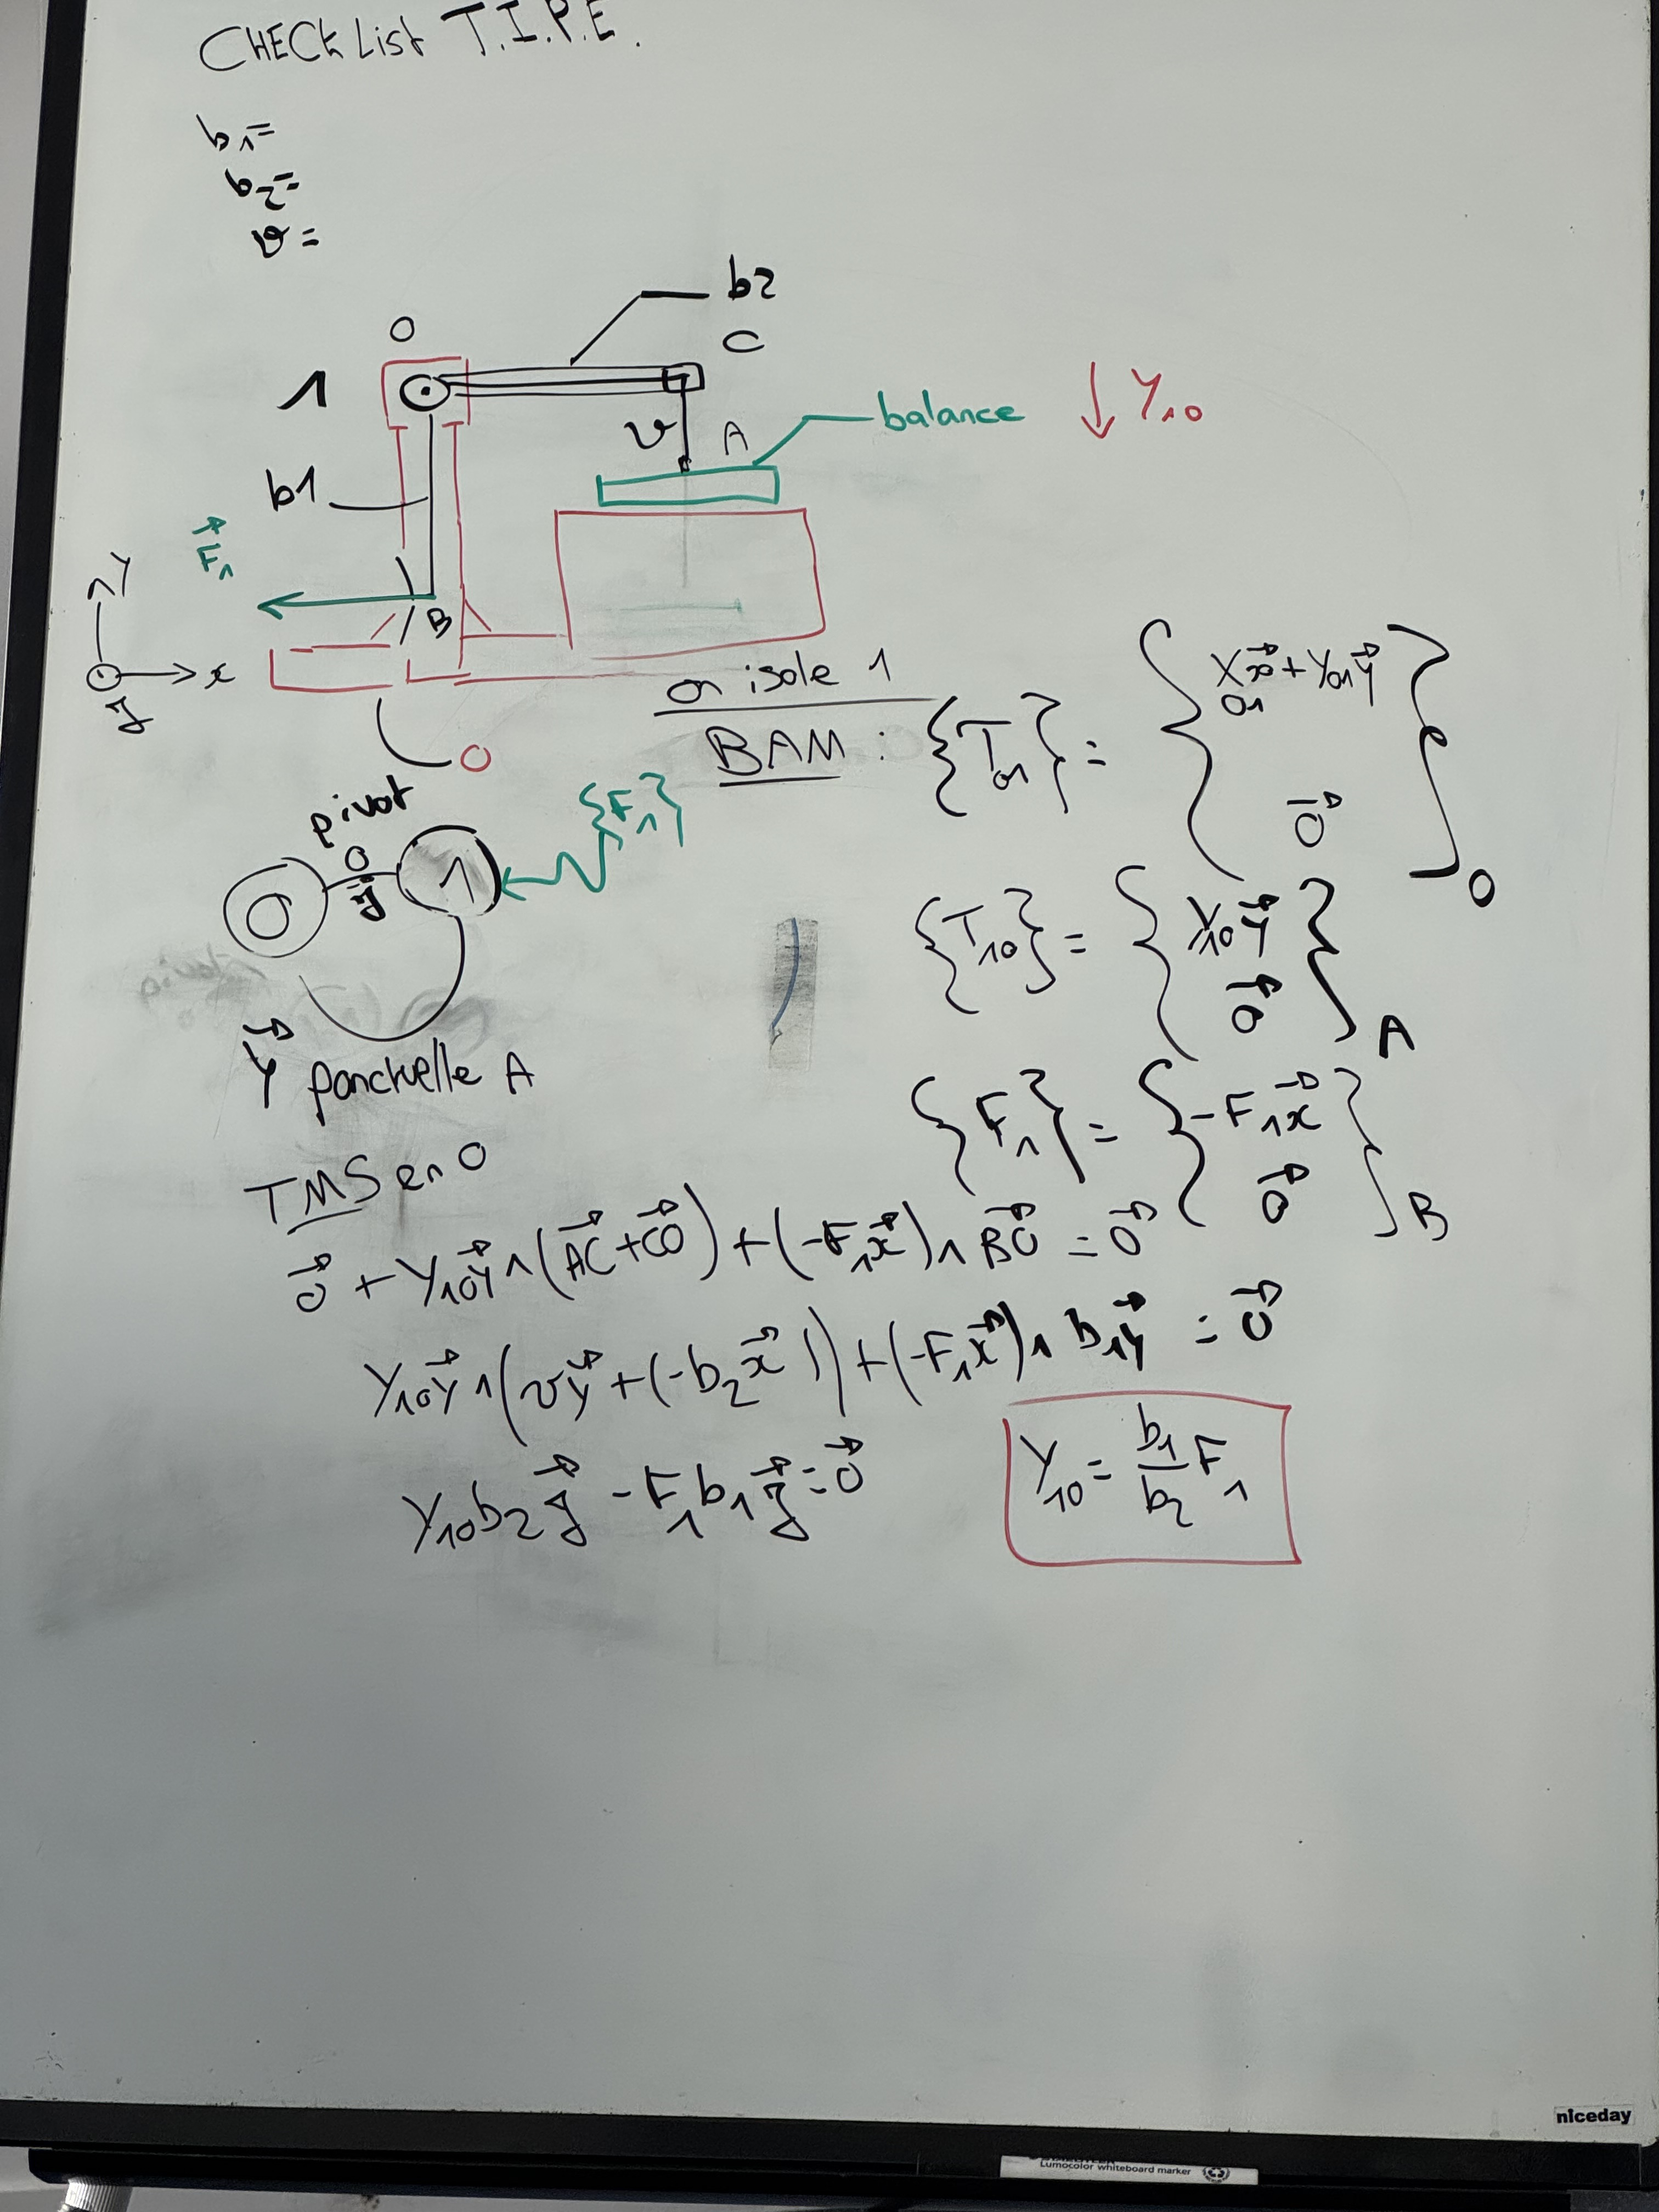
\includegraphics[height=0.85\textheight,width=\textwidth,keepaspectratio]{calculstatique.jpg}
  \par\vspace{2pt}{\scriptsize \textit{Modèle statique du banc en « L »}}
\end{frame}

\begin{frame}{Réalisation du banc : Frettage, soudure et peinture}
  \begin{columns}
    \column{0.33\textwidth}
    \centering
    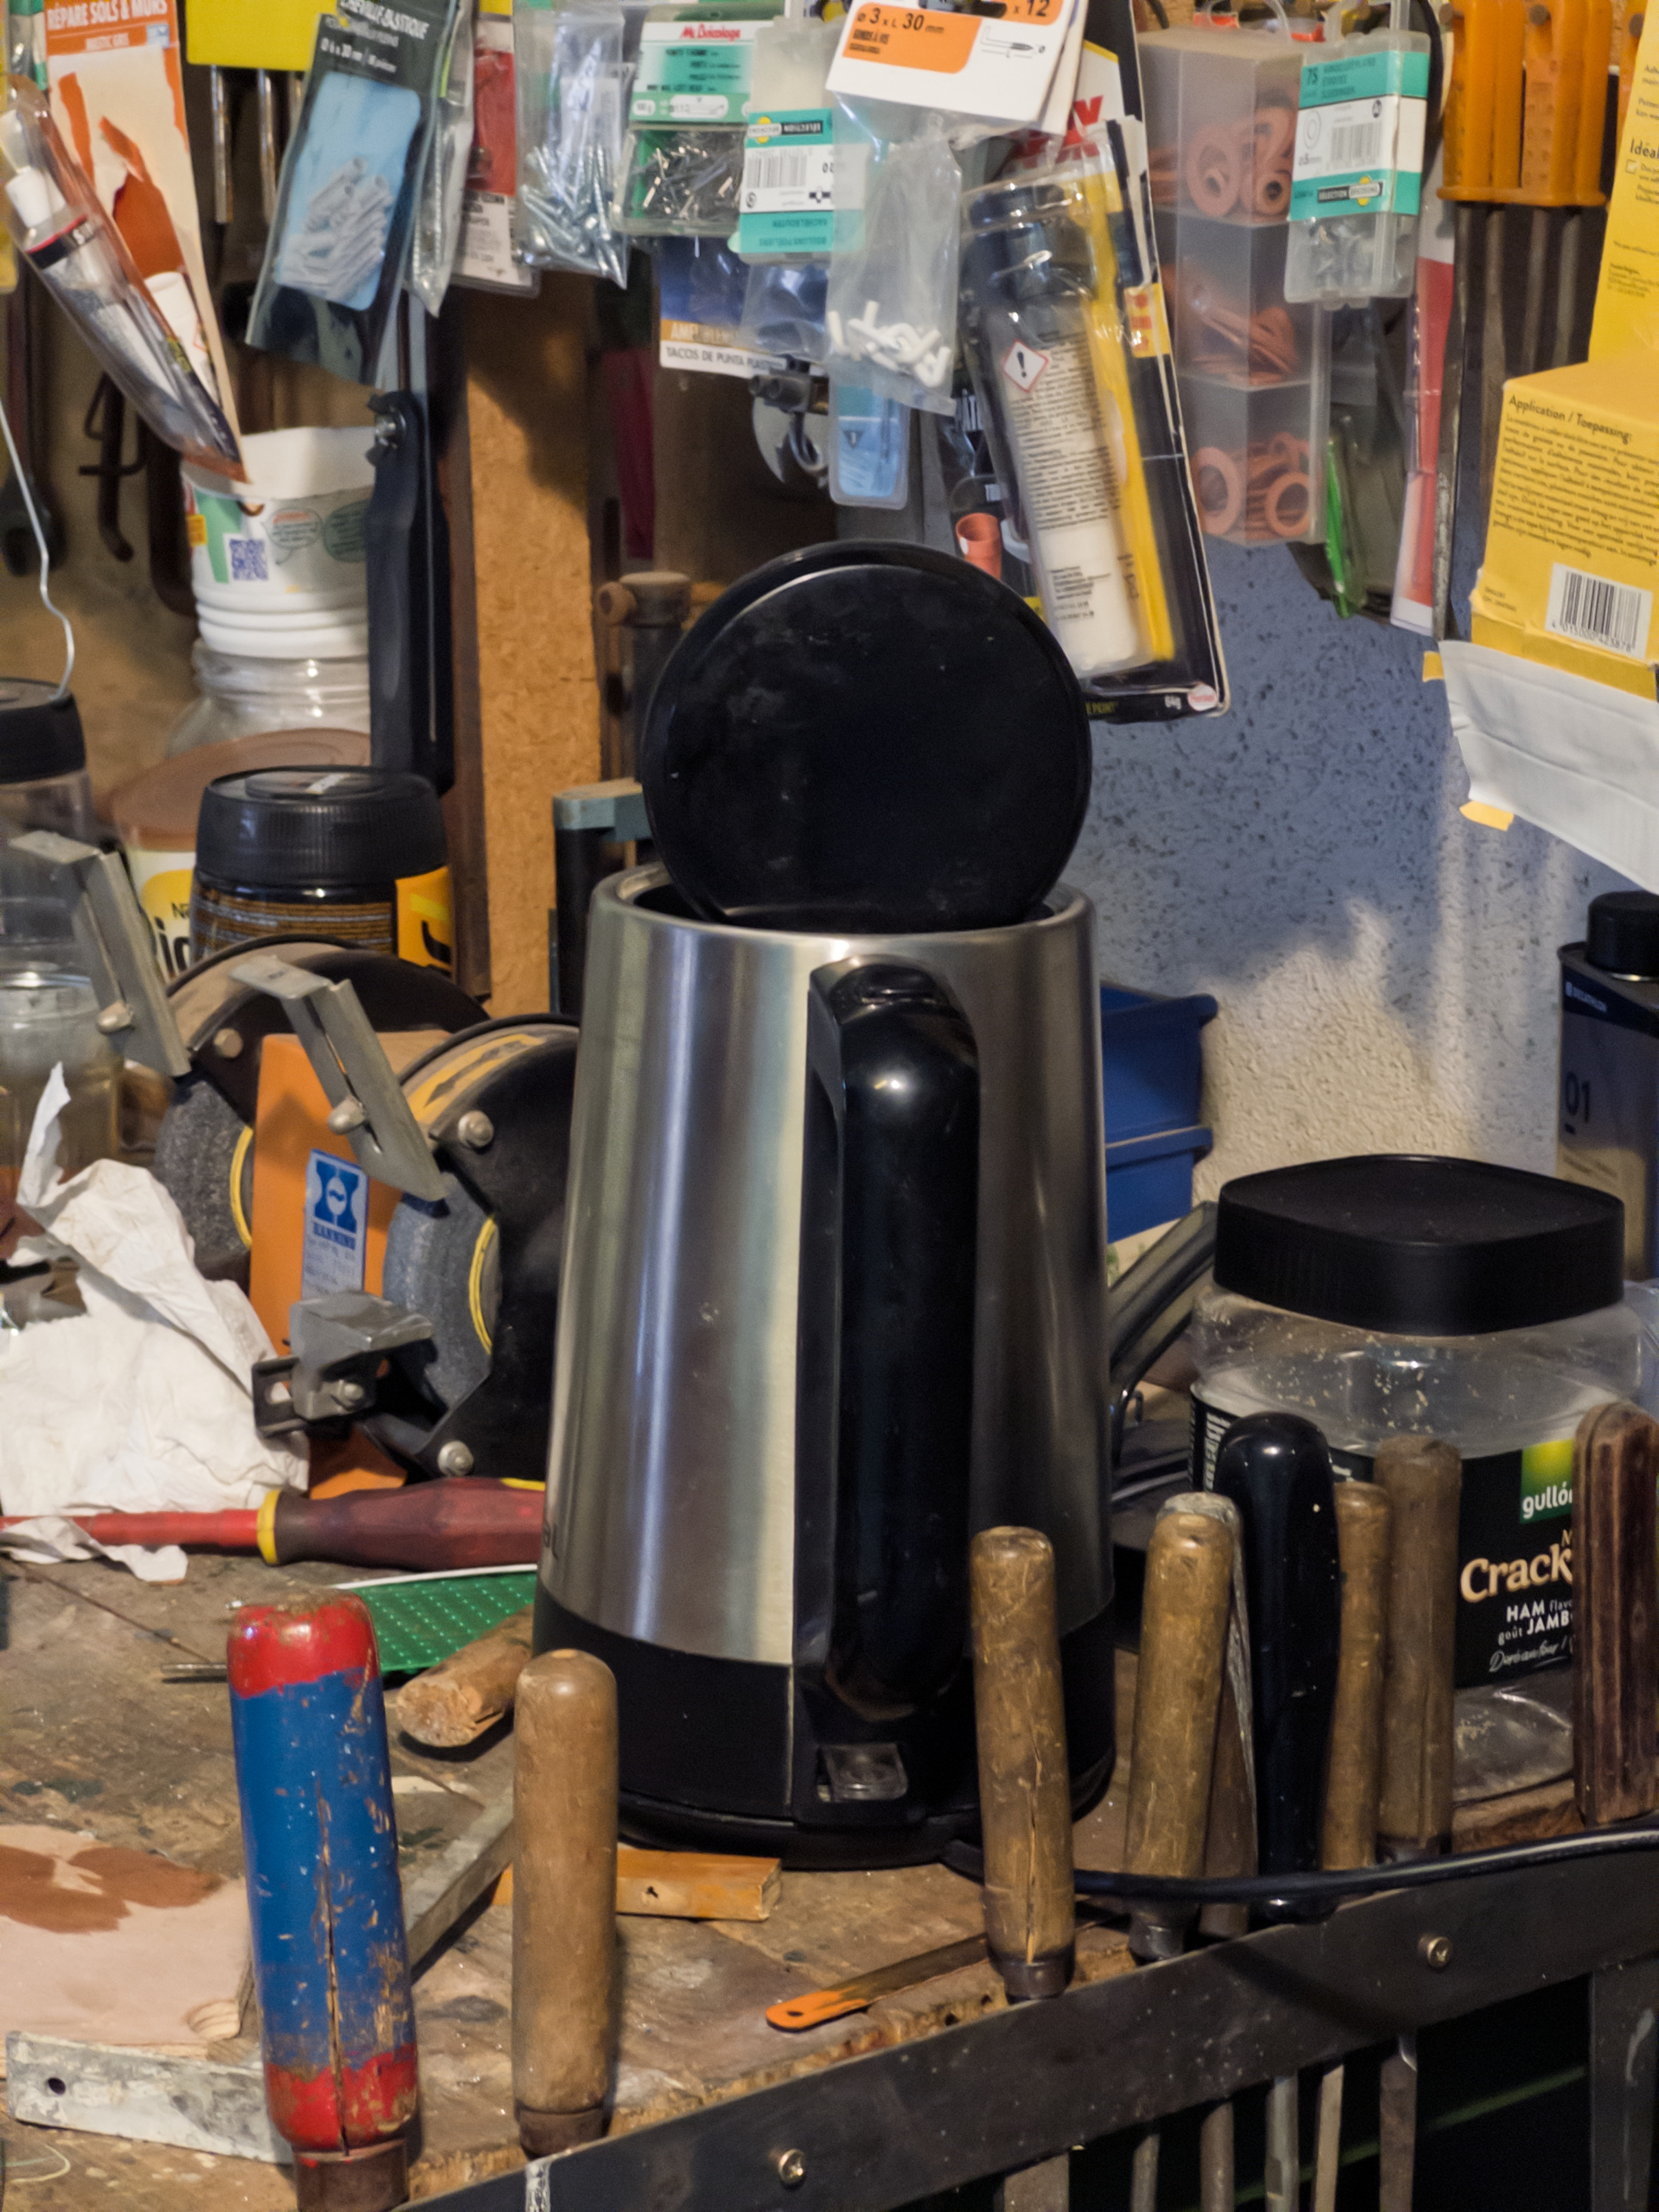
\includegraphics[width=0.9\textwidth,height=0.45\textheight,keepaspectratio]{bouilloire.JPG}
    \par\vspace{2pt}{\scriptsize \textit{Dilatation du tube aluminium}}
    \vspace{0.2cm}
    \begin{itemize}
      \item \scriptsize \textbf{Frettage :} Tube en alu dilaté (pas sur que ce soit nécessaire au final) dans l'eau bouillante pour une insertion parfaitement serrée du pivot.
    \end{itemize}

    \column{0.33\textwidth}
    \centering
    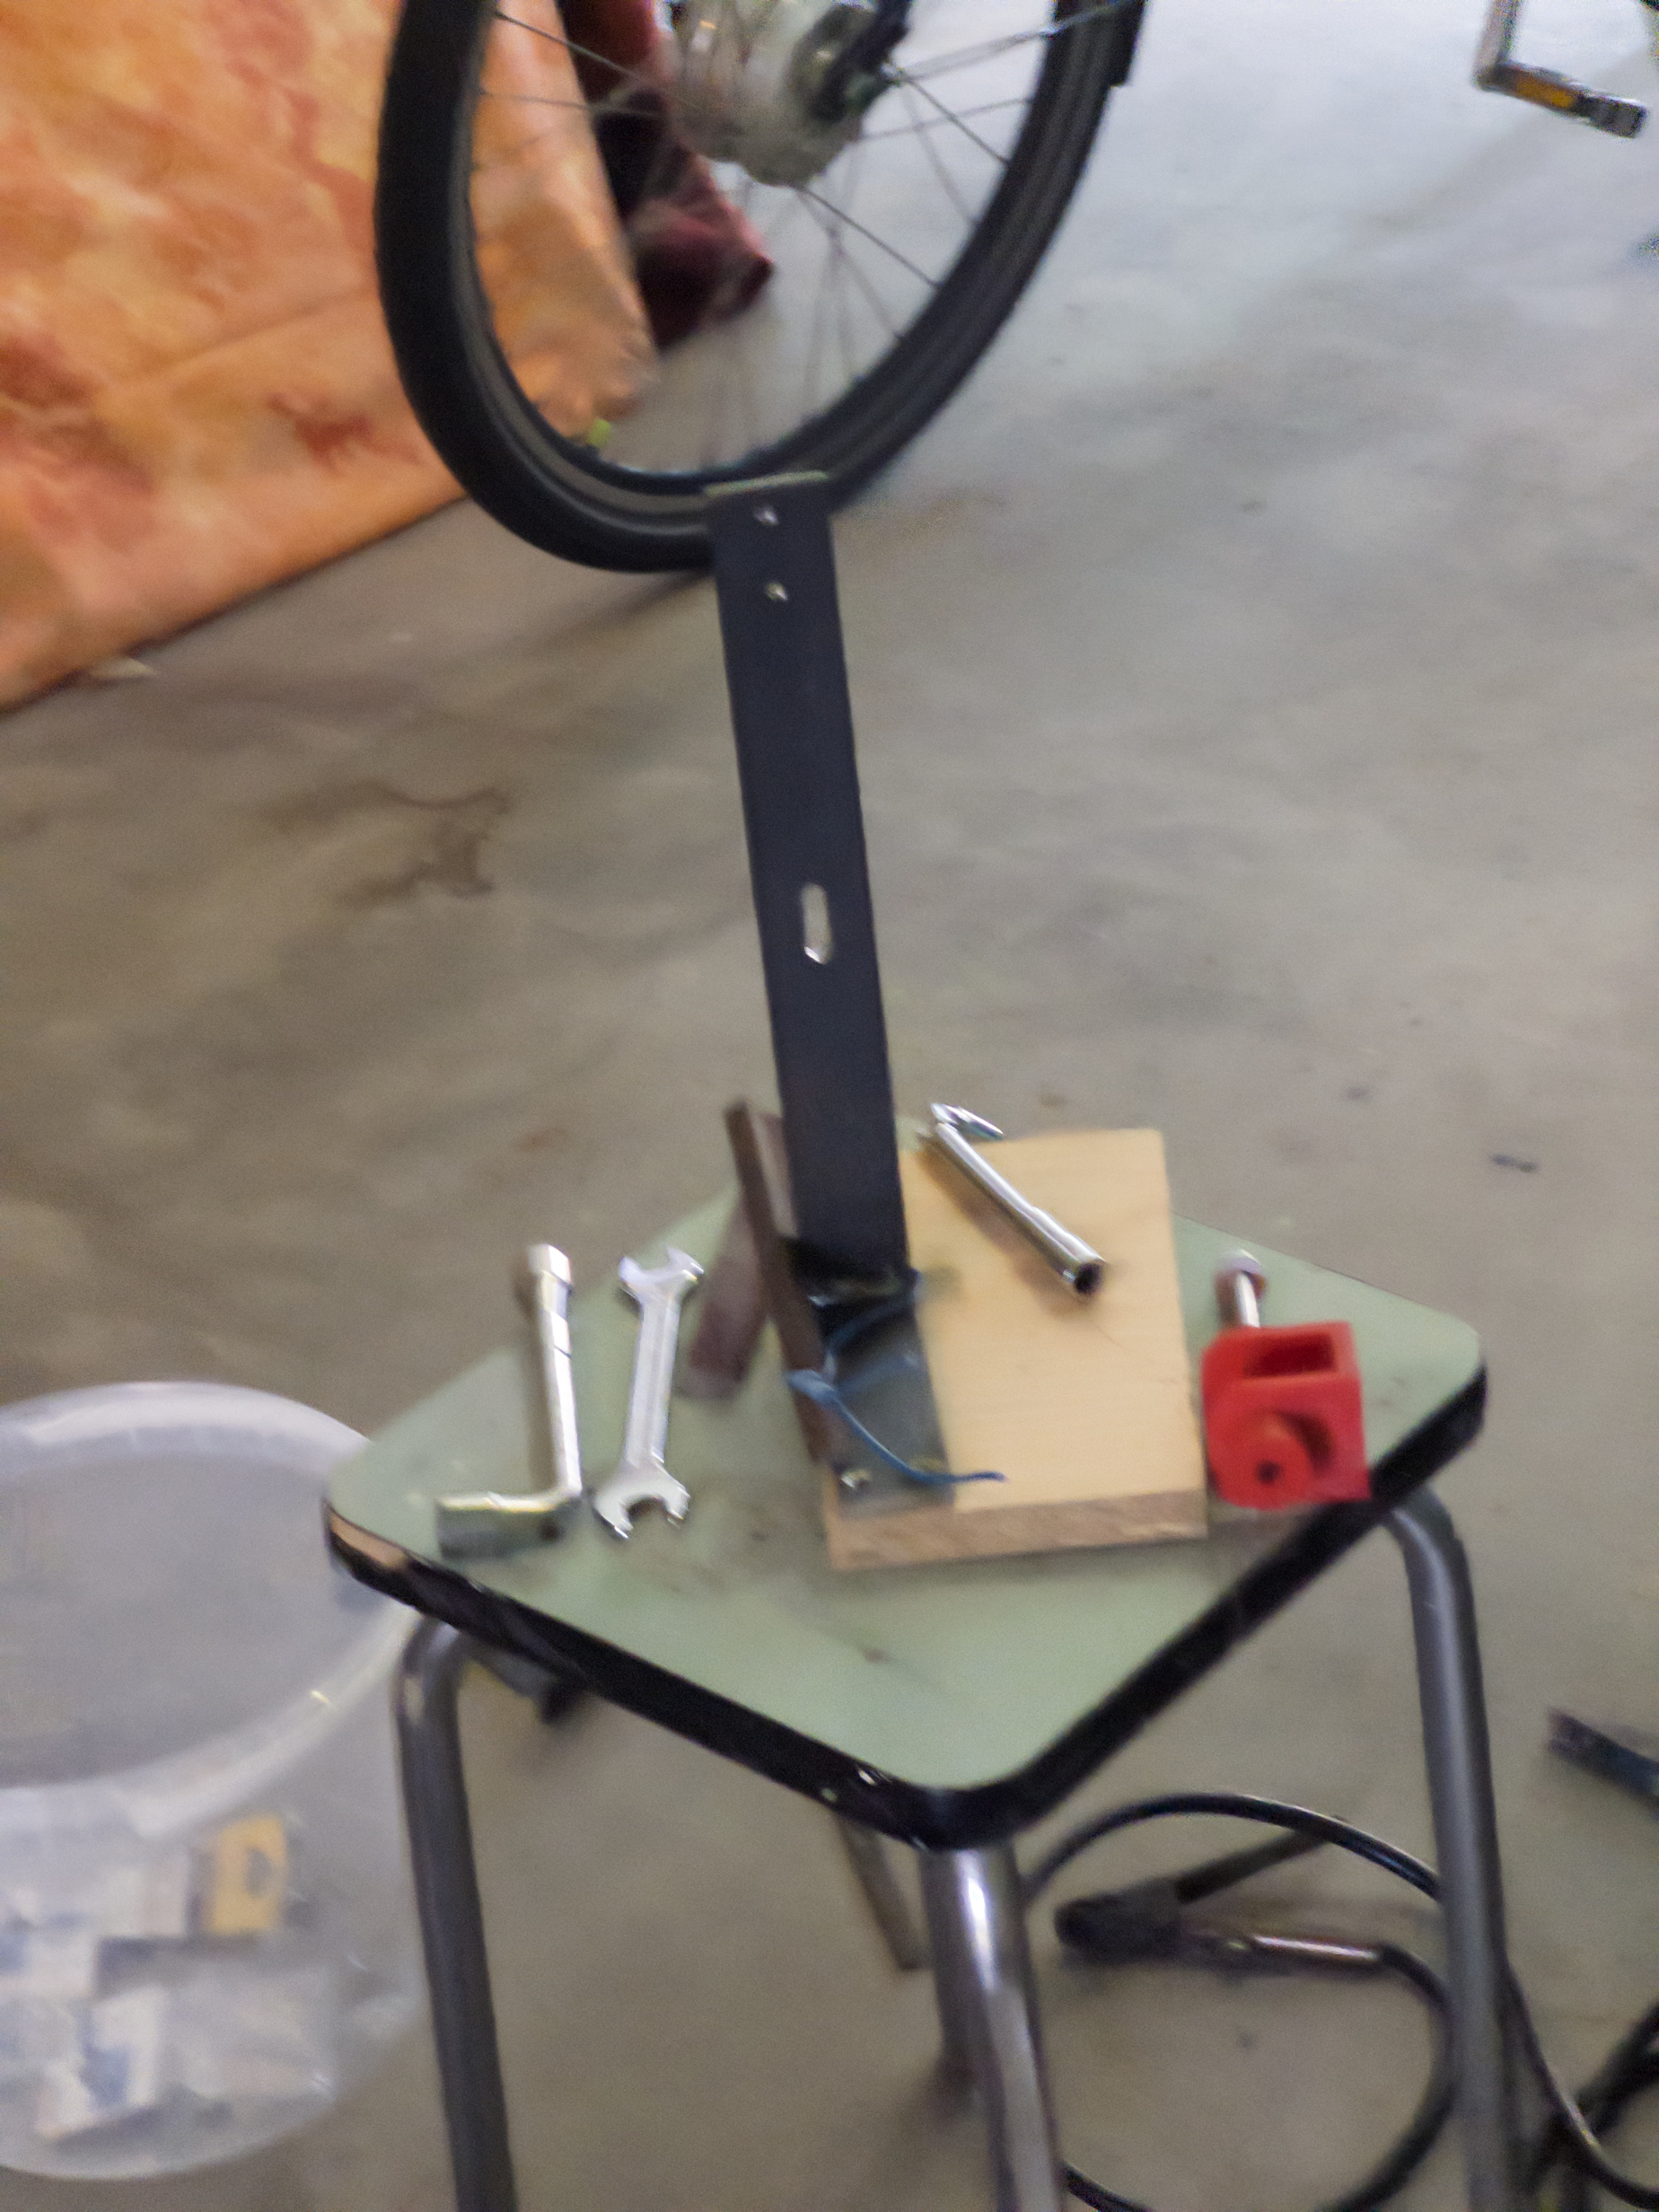
\includegraphics[width=0.9\textwidth,height=0.45\textheight,keepaspectratio]{soudure1.JPG}
    \par\vspace{2pt}{\scriptsize \textit{Soudure du bâti en acier}}
    \vspace{0.2cm}
    \begin{itemize}
      \item \scriptsize \textbf{Assemblage :} Soudure à l'arc du support fixe pour garantir une grande rigidité face aux vibrations.
    \end{itemize}

    \column{0.33\textwidth}
    \centering
    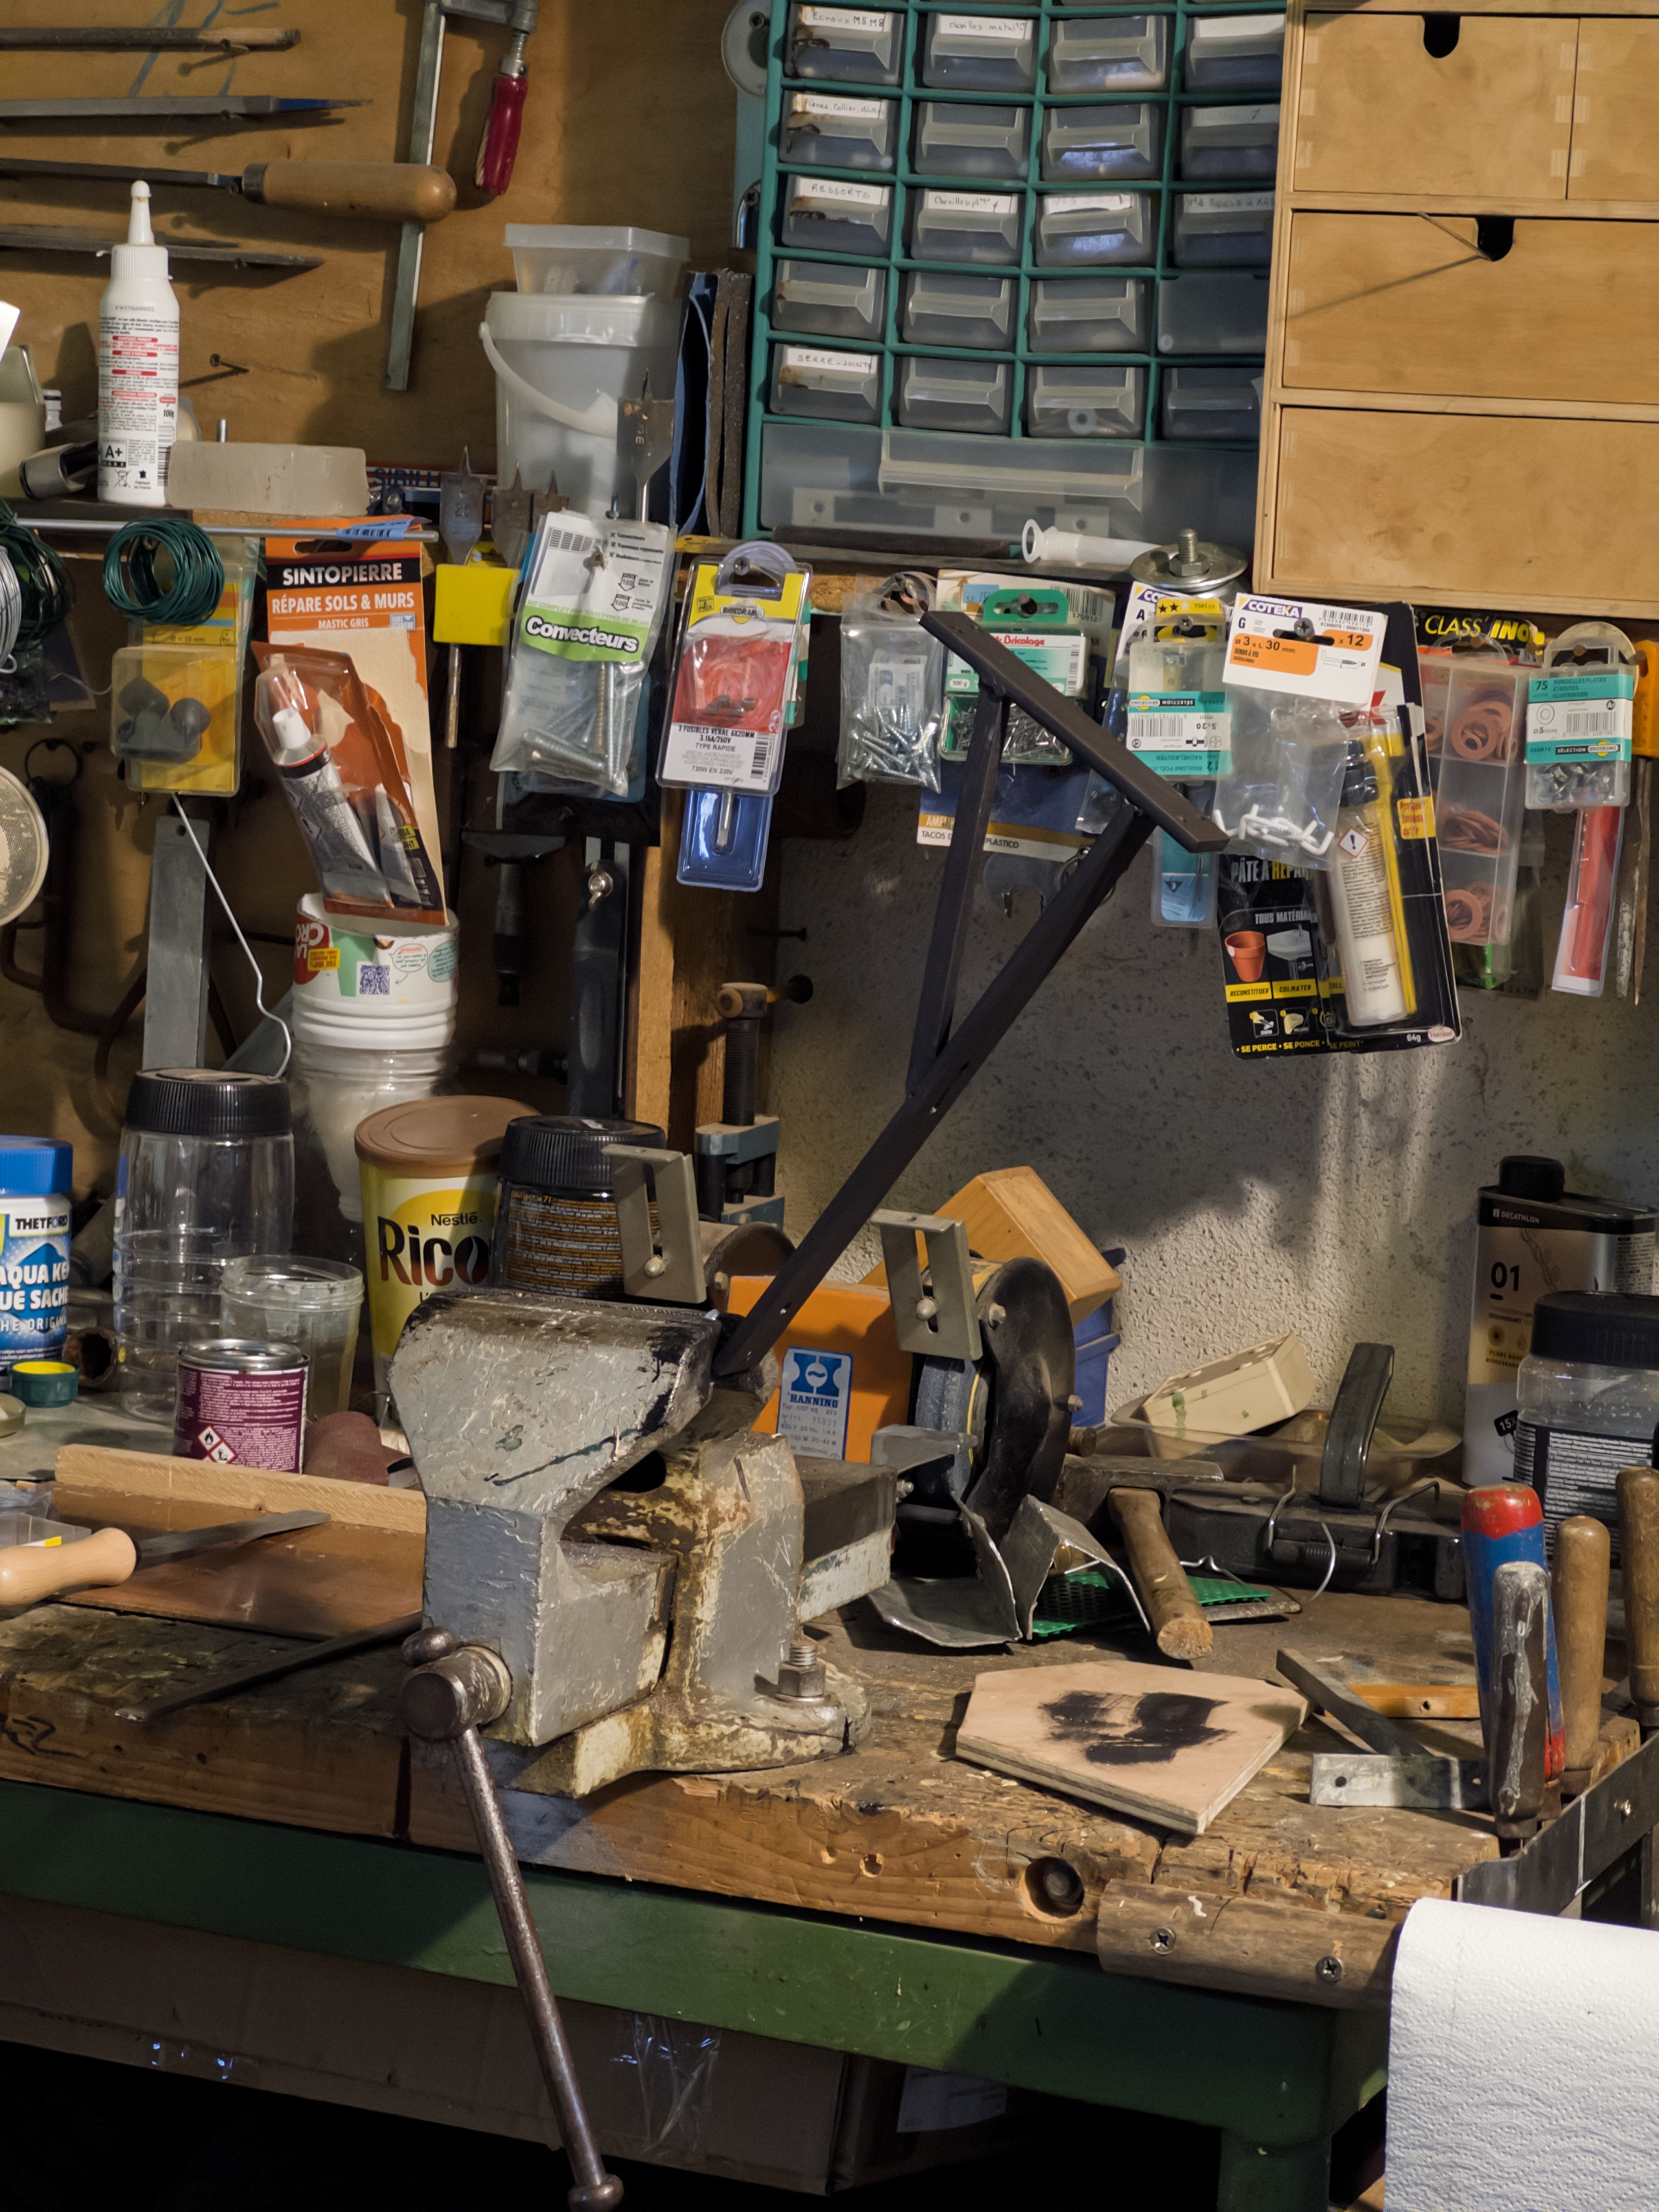
\includegraphics[width=0.9\textwidth,height=0.45\textheight,keepaspectratio]{peinture.JPG}
    \par\vspace{2pt}{\scriptsize \textit{Bâti finalisé et peint}}
    \vspace{0.2cm}
    \begin{itemize}
      \item \scriptsize \textbf{Finition :} Peinture.
    \end{itemize}
  \end{columns}
\end{frame}

\begin{frame}{Alimentation et commande (Travail des vacances)}
  \begin{columns}
    \column{0.55\textwidth}
    \textbf{Sécurisation et robustesse du système :}
    \begin{itemize}
      \item \textbf{Alimentation : } Utilisation d'une batterie LiPo 4S pour fournir les $\sim 40\text{ A}$ nécessaires (hors de portée d'une alimentation de laboratoire classique).
      \item \textbf{Commande du Moteur :} Un Raspberry Pi 4 (ou carte Arduino) génère un signal PWM pour l'ESC (le contrôleur du moteur).
    \end{itemize}

    \column{0.45\textwidth}
    \begin{alertblock}{Sécurité absolue du dispositif}
      \small
      À $25\,000\text{ tr/min}$, vitesse en bout de pale :
      \[
        V_{\text{bout}} = \omega \cdot R \approx 166\text{ m/s} \quad (\approx 600\text{ km/h})
      \]
      \textbf{Dispositifs obligatoires :}
      \begin{itemize}
        \item Coupure d'urgence matérielle et logicielle.
        \item \textbf{Cage de protection} (polycarbonate).
      \end{itemize}
    \end{alertblock}
  \end{columns}
\end{frame}

% =========================================================================
\section{Objectifs pour la 2\texorpdfstring{\textsuperscript{ème}}{ème} Année}
% =========================================================================

\begin{frame}{Objectifs et suites du TIPE}
  \textbf{Les prochaines étapes :}
  \begin{itemize}
    \item pivot en avec roulement
    \item Faire la cage de protection.
    \item Finir de construire le banc d'essai.
    \item Souder le moteur à l'ESC.
    \item Écrire le script Arduino pour gérer le dispositif.
    \item Tester avec la balance puis intégrer la cellule de charge (réfléchir à son placement).
    \item Tester la rigidité des pales.
  \end{itemize}
\end{frame}

% =========================================================================
\appendix
\section{Annexes}
% =========================================================================

\begin{frame}{Annexe : Impression 3D (Imprimante et Pièces)}
  \begin{columns}
    \column{0.33\textwidth}
    \centering
    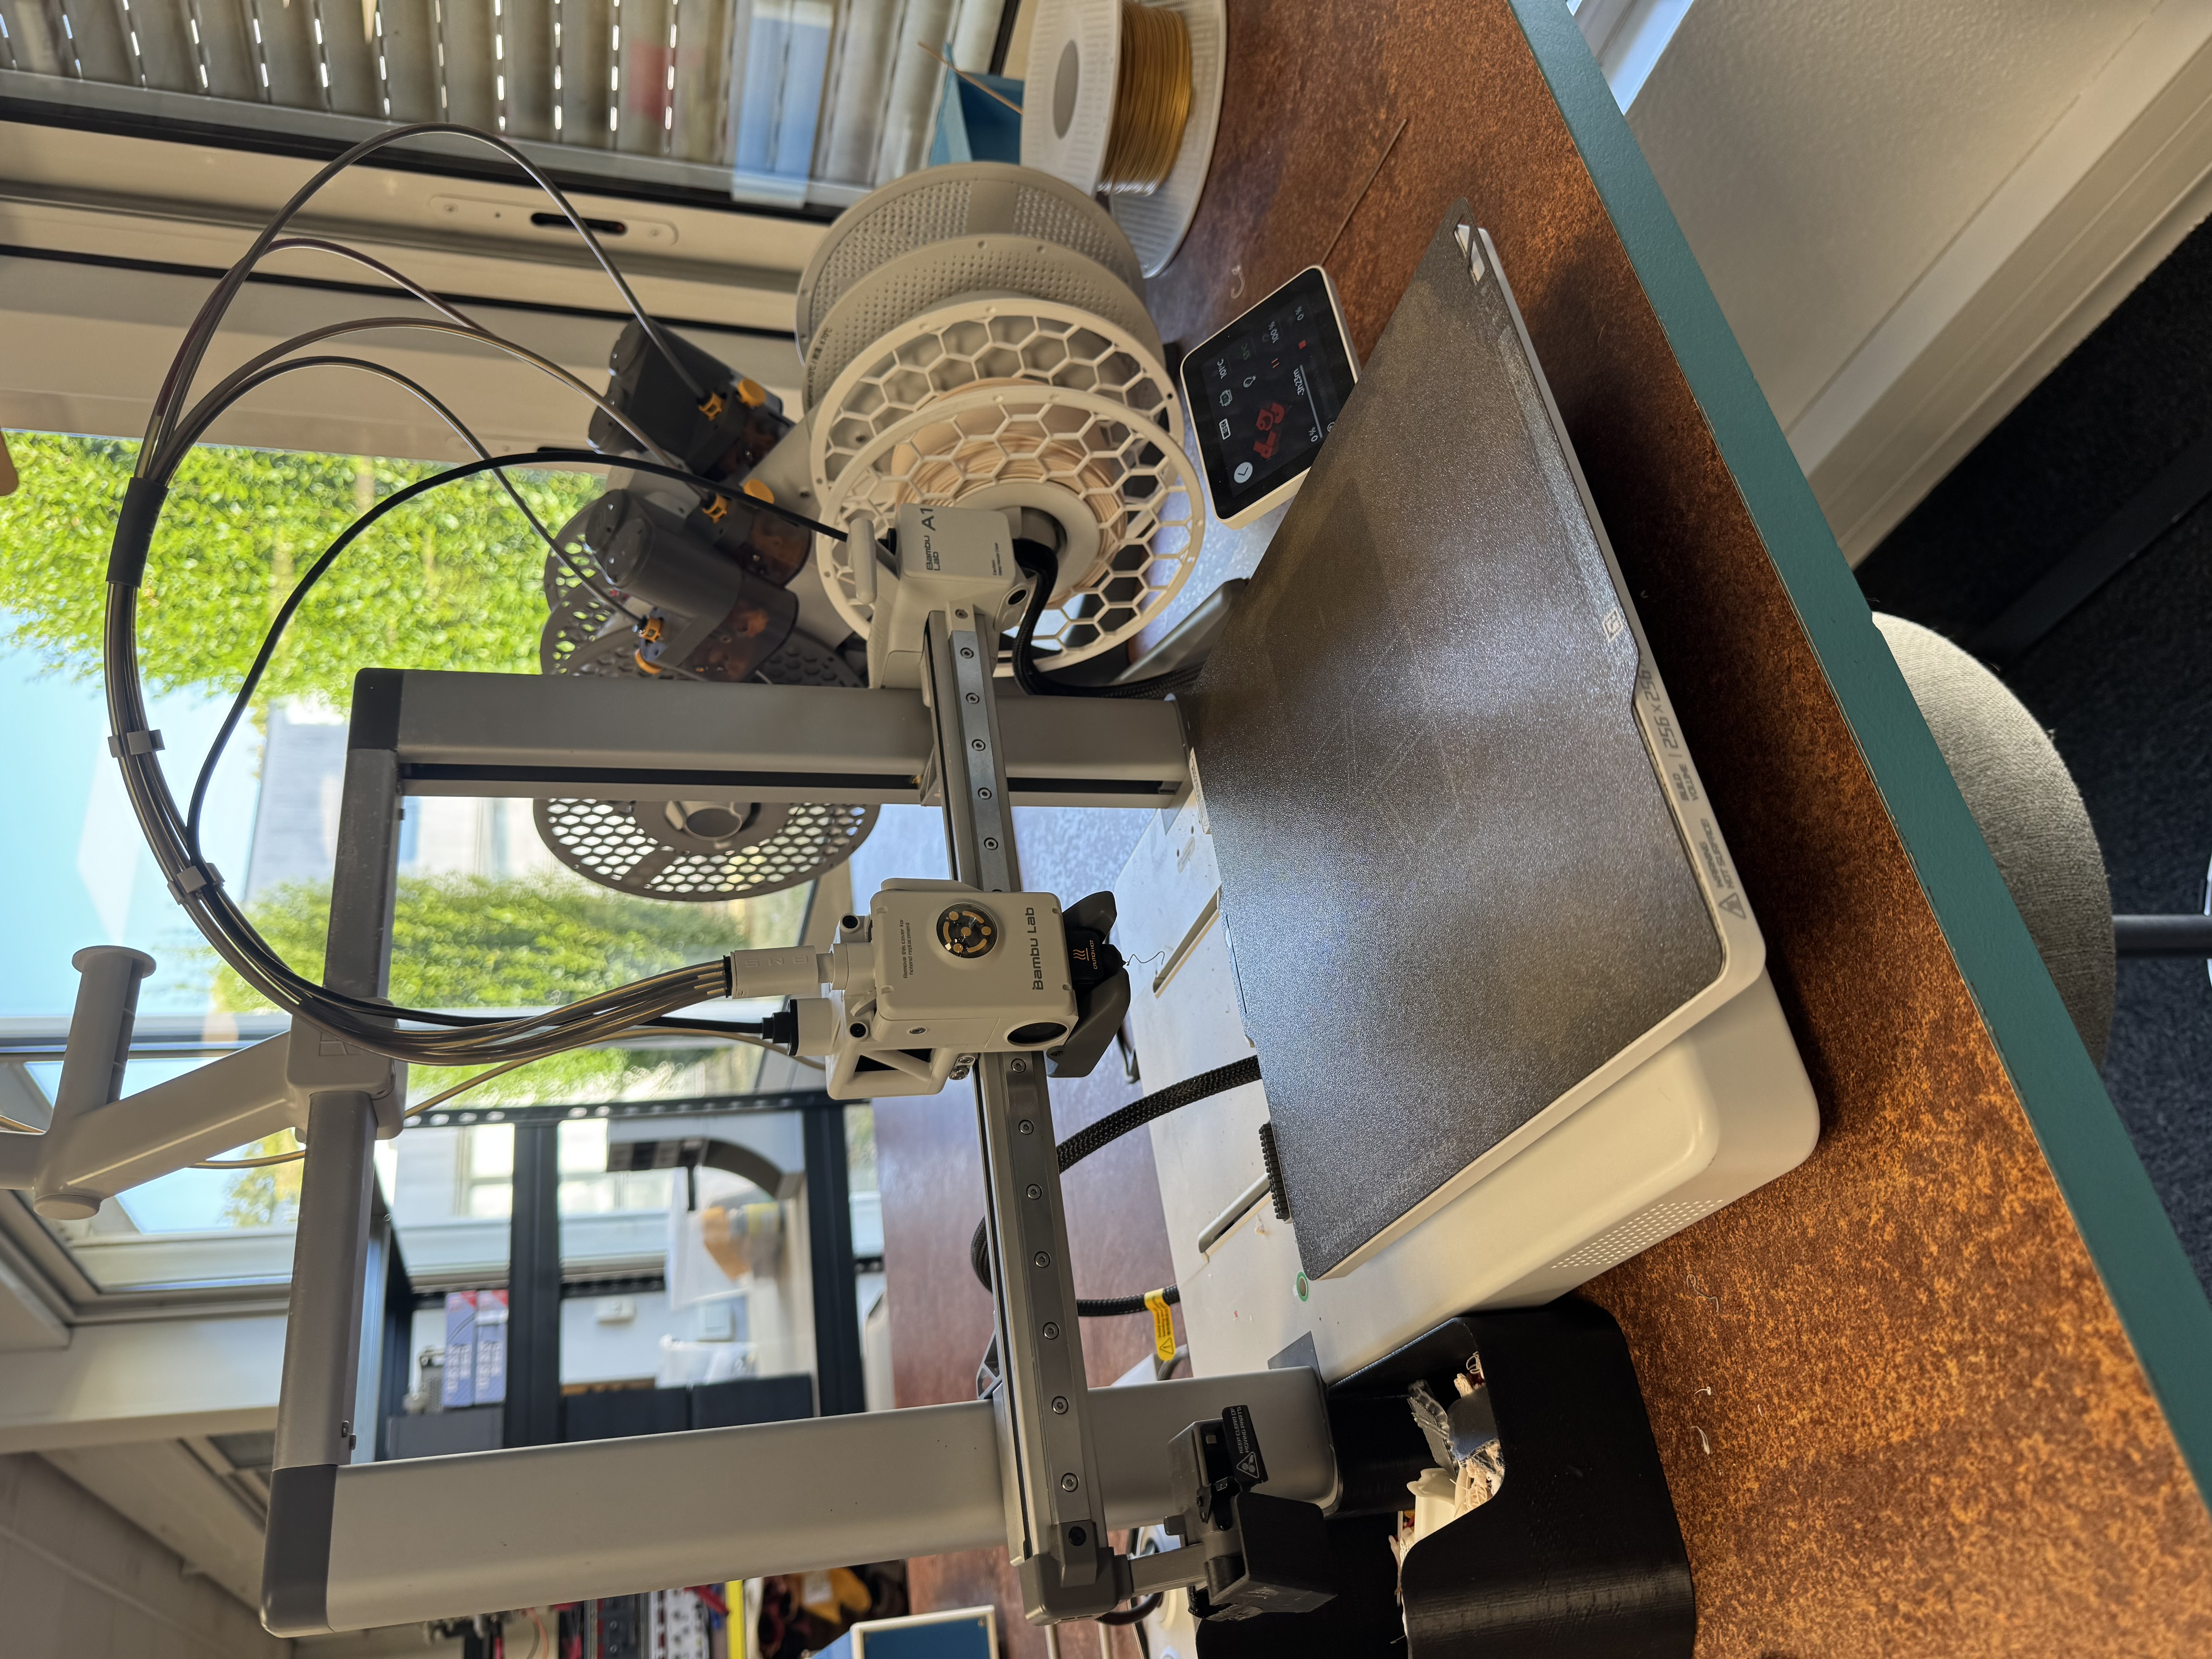
\includegraphics[width=\textwidth,height=0.4\textheight,keepaspectratio]{imprimante.jpg}
    \par\vspace{2pt}{\scriptsize \textit{Imprimante 3D}}

    \column{0.33\textwidth}
    \centering
    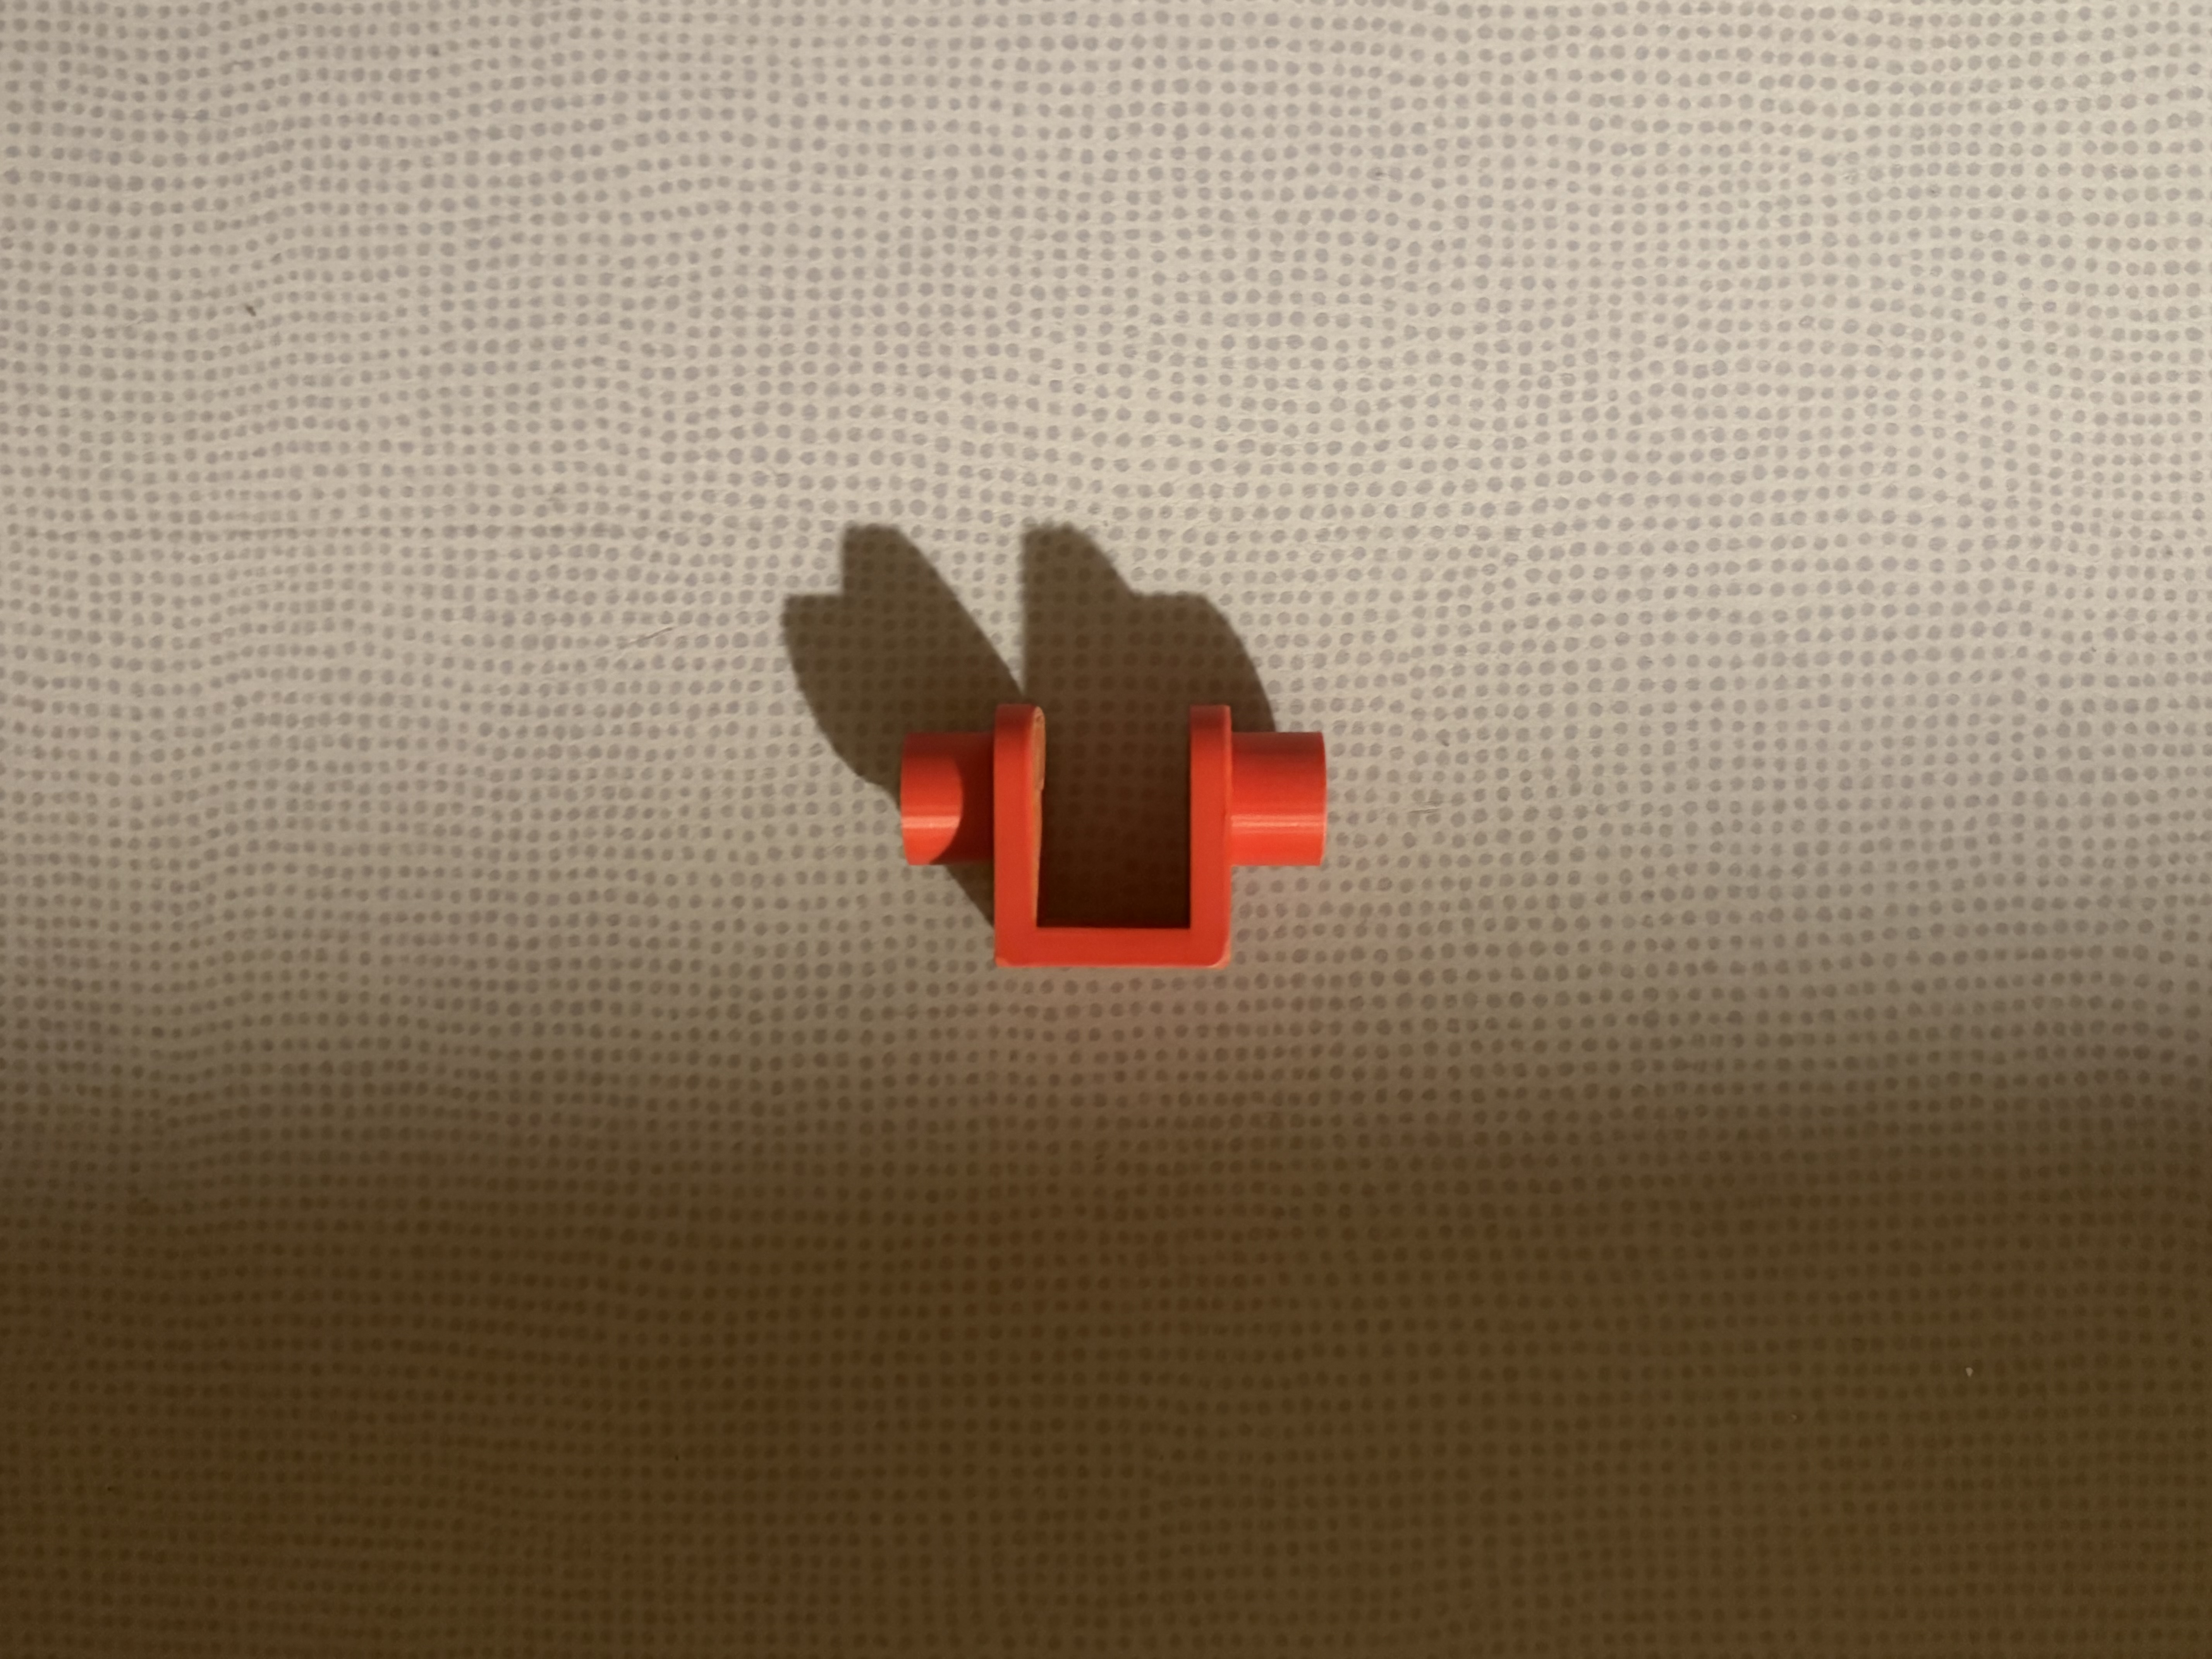
\includegraphics[width=\textwidth,height=0.4\textheight,keepaspectratio]{piece1.jpg}
    \par\vspace{2pt}{\scriptsize \textit{Pièce 1}}
    \vspace{0.2cm}
    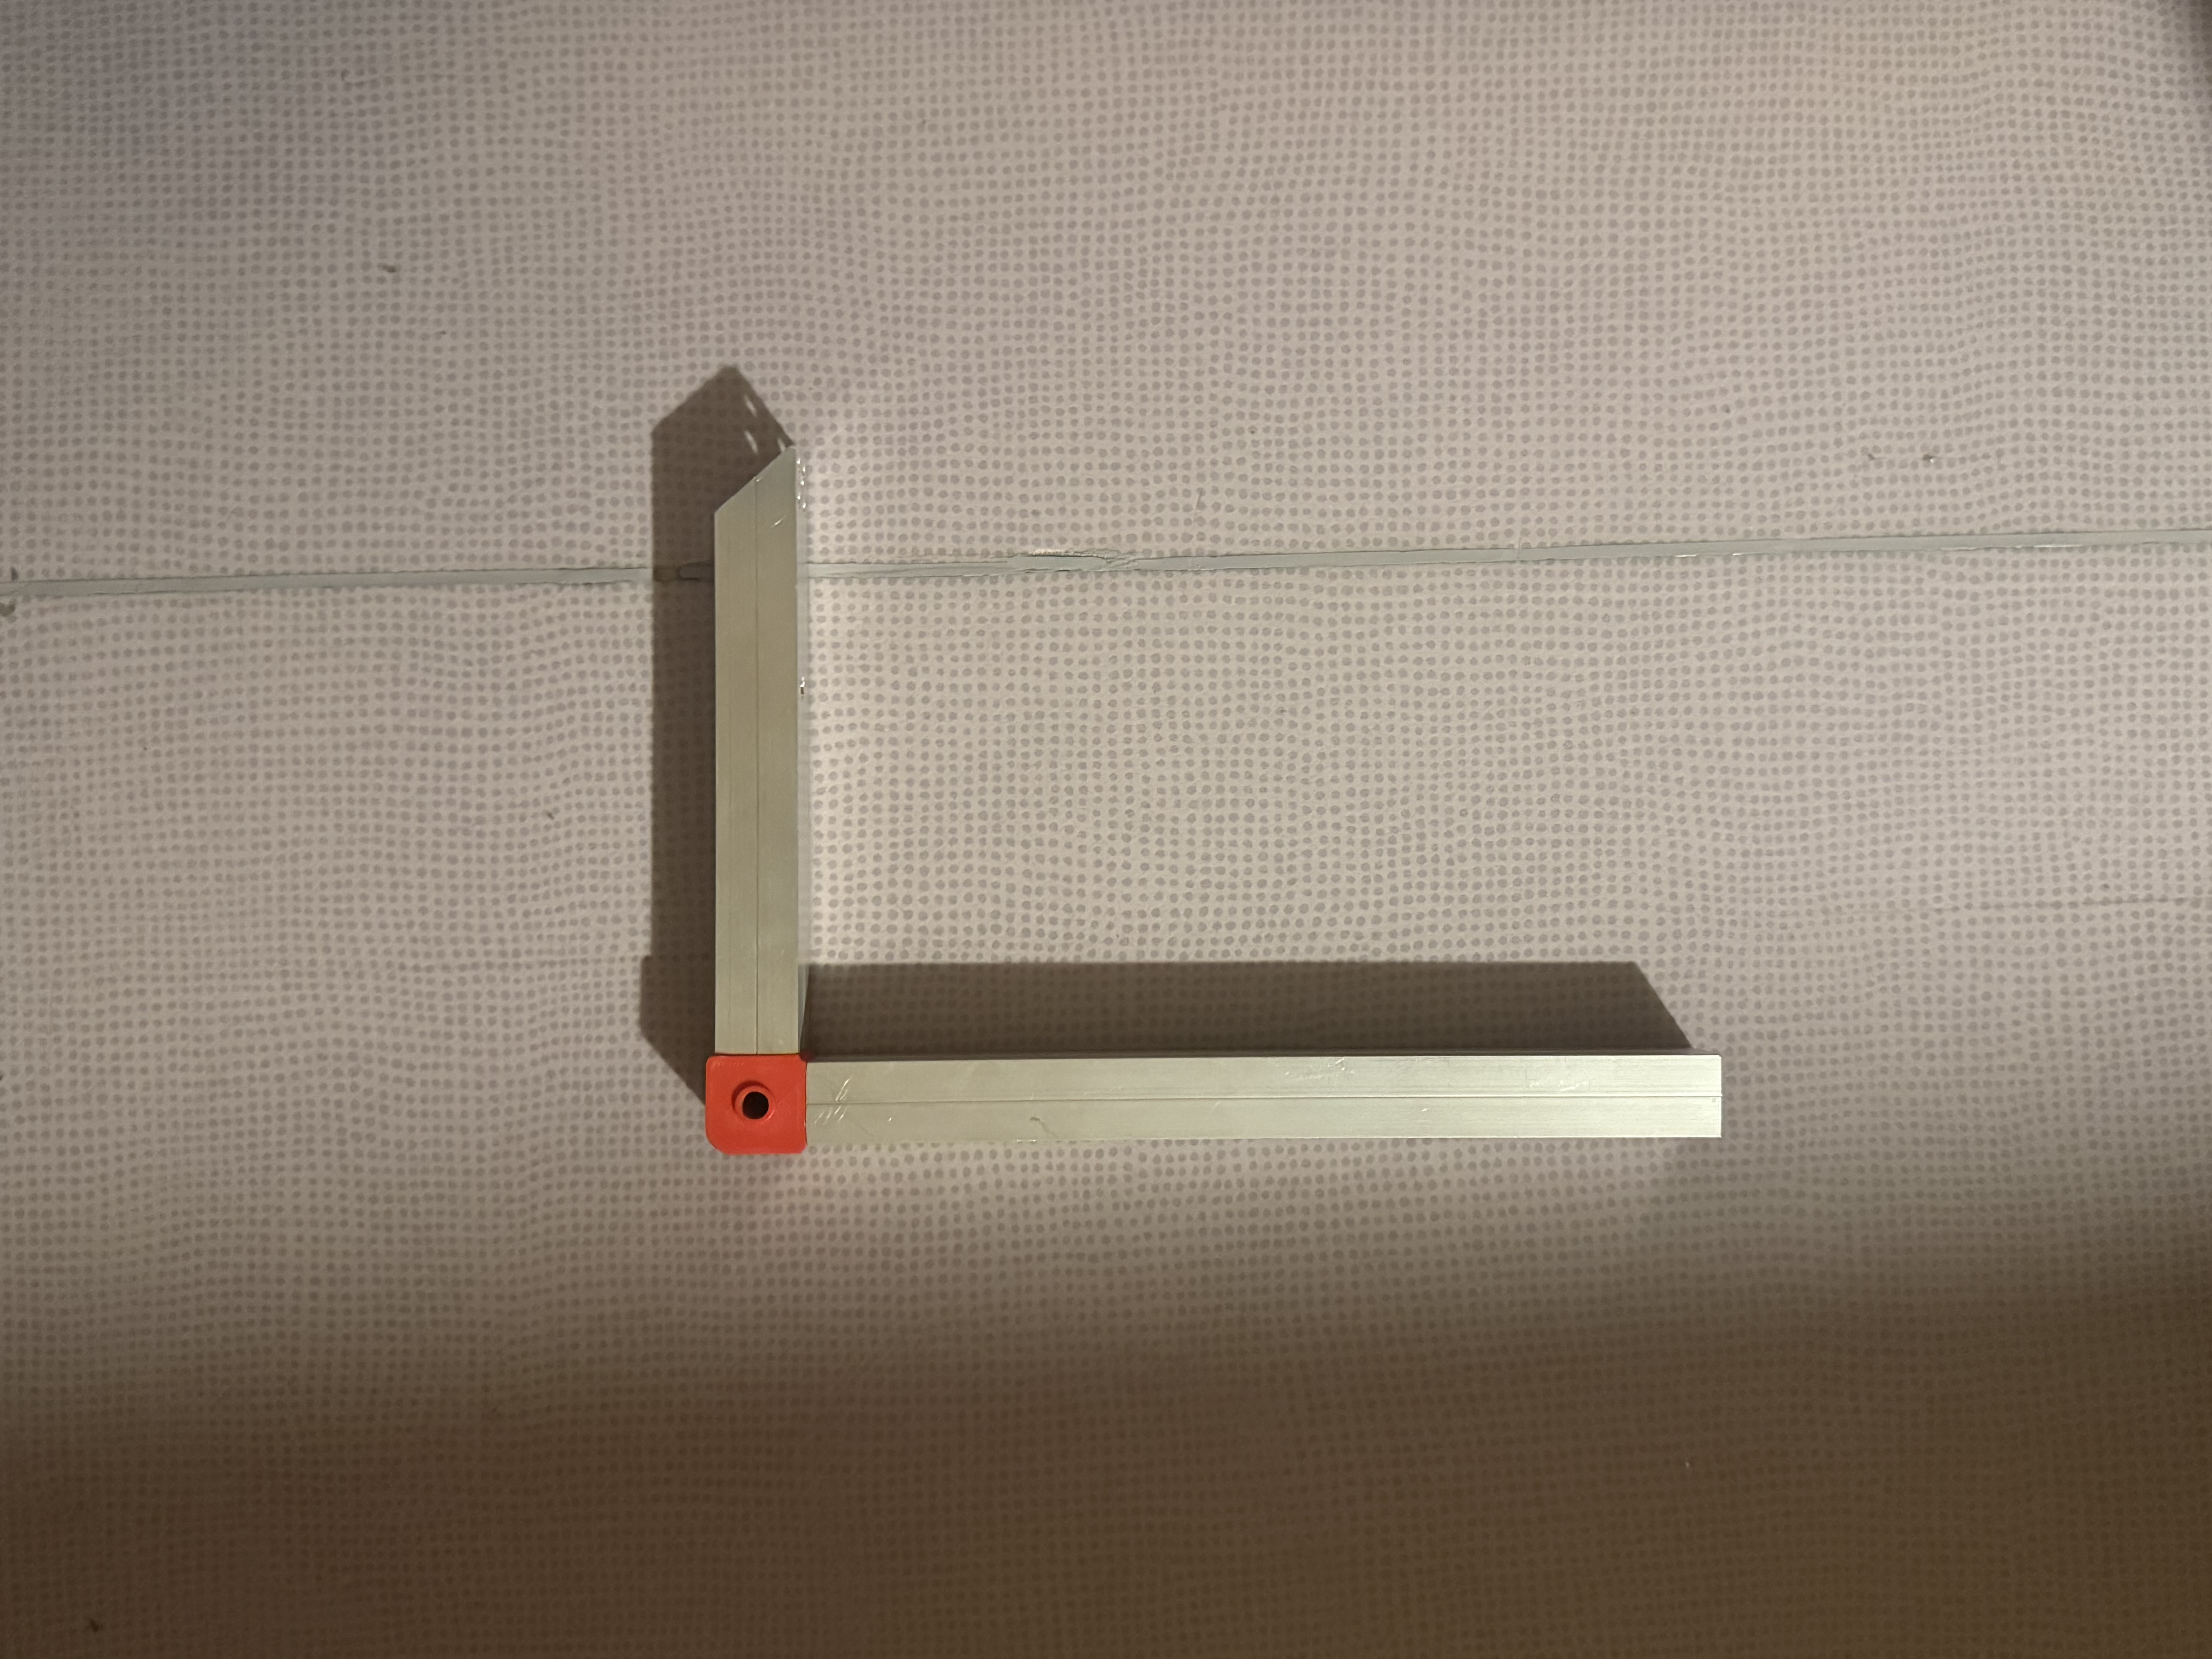
\includegraphics[width=\textwidth,height=0.4\textheight,keepaspectratio]{piece2.jpg}
    \par\vspace{2pt}{\scriptsize \textit{Pièce 2}}

    \column{0.33\textwidth}
    \centering
    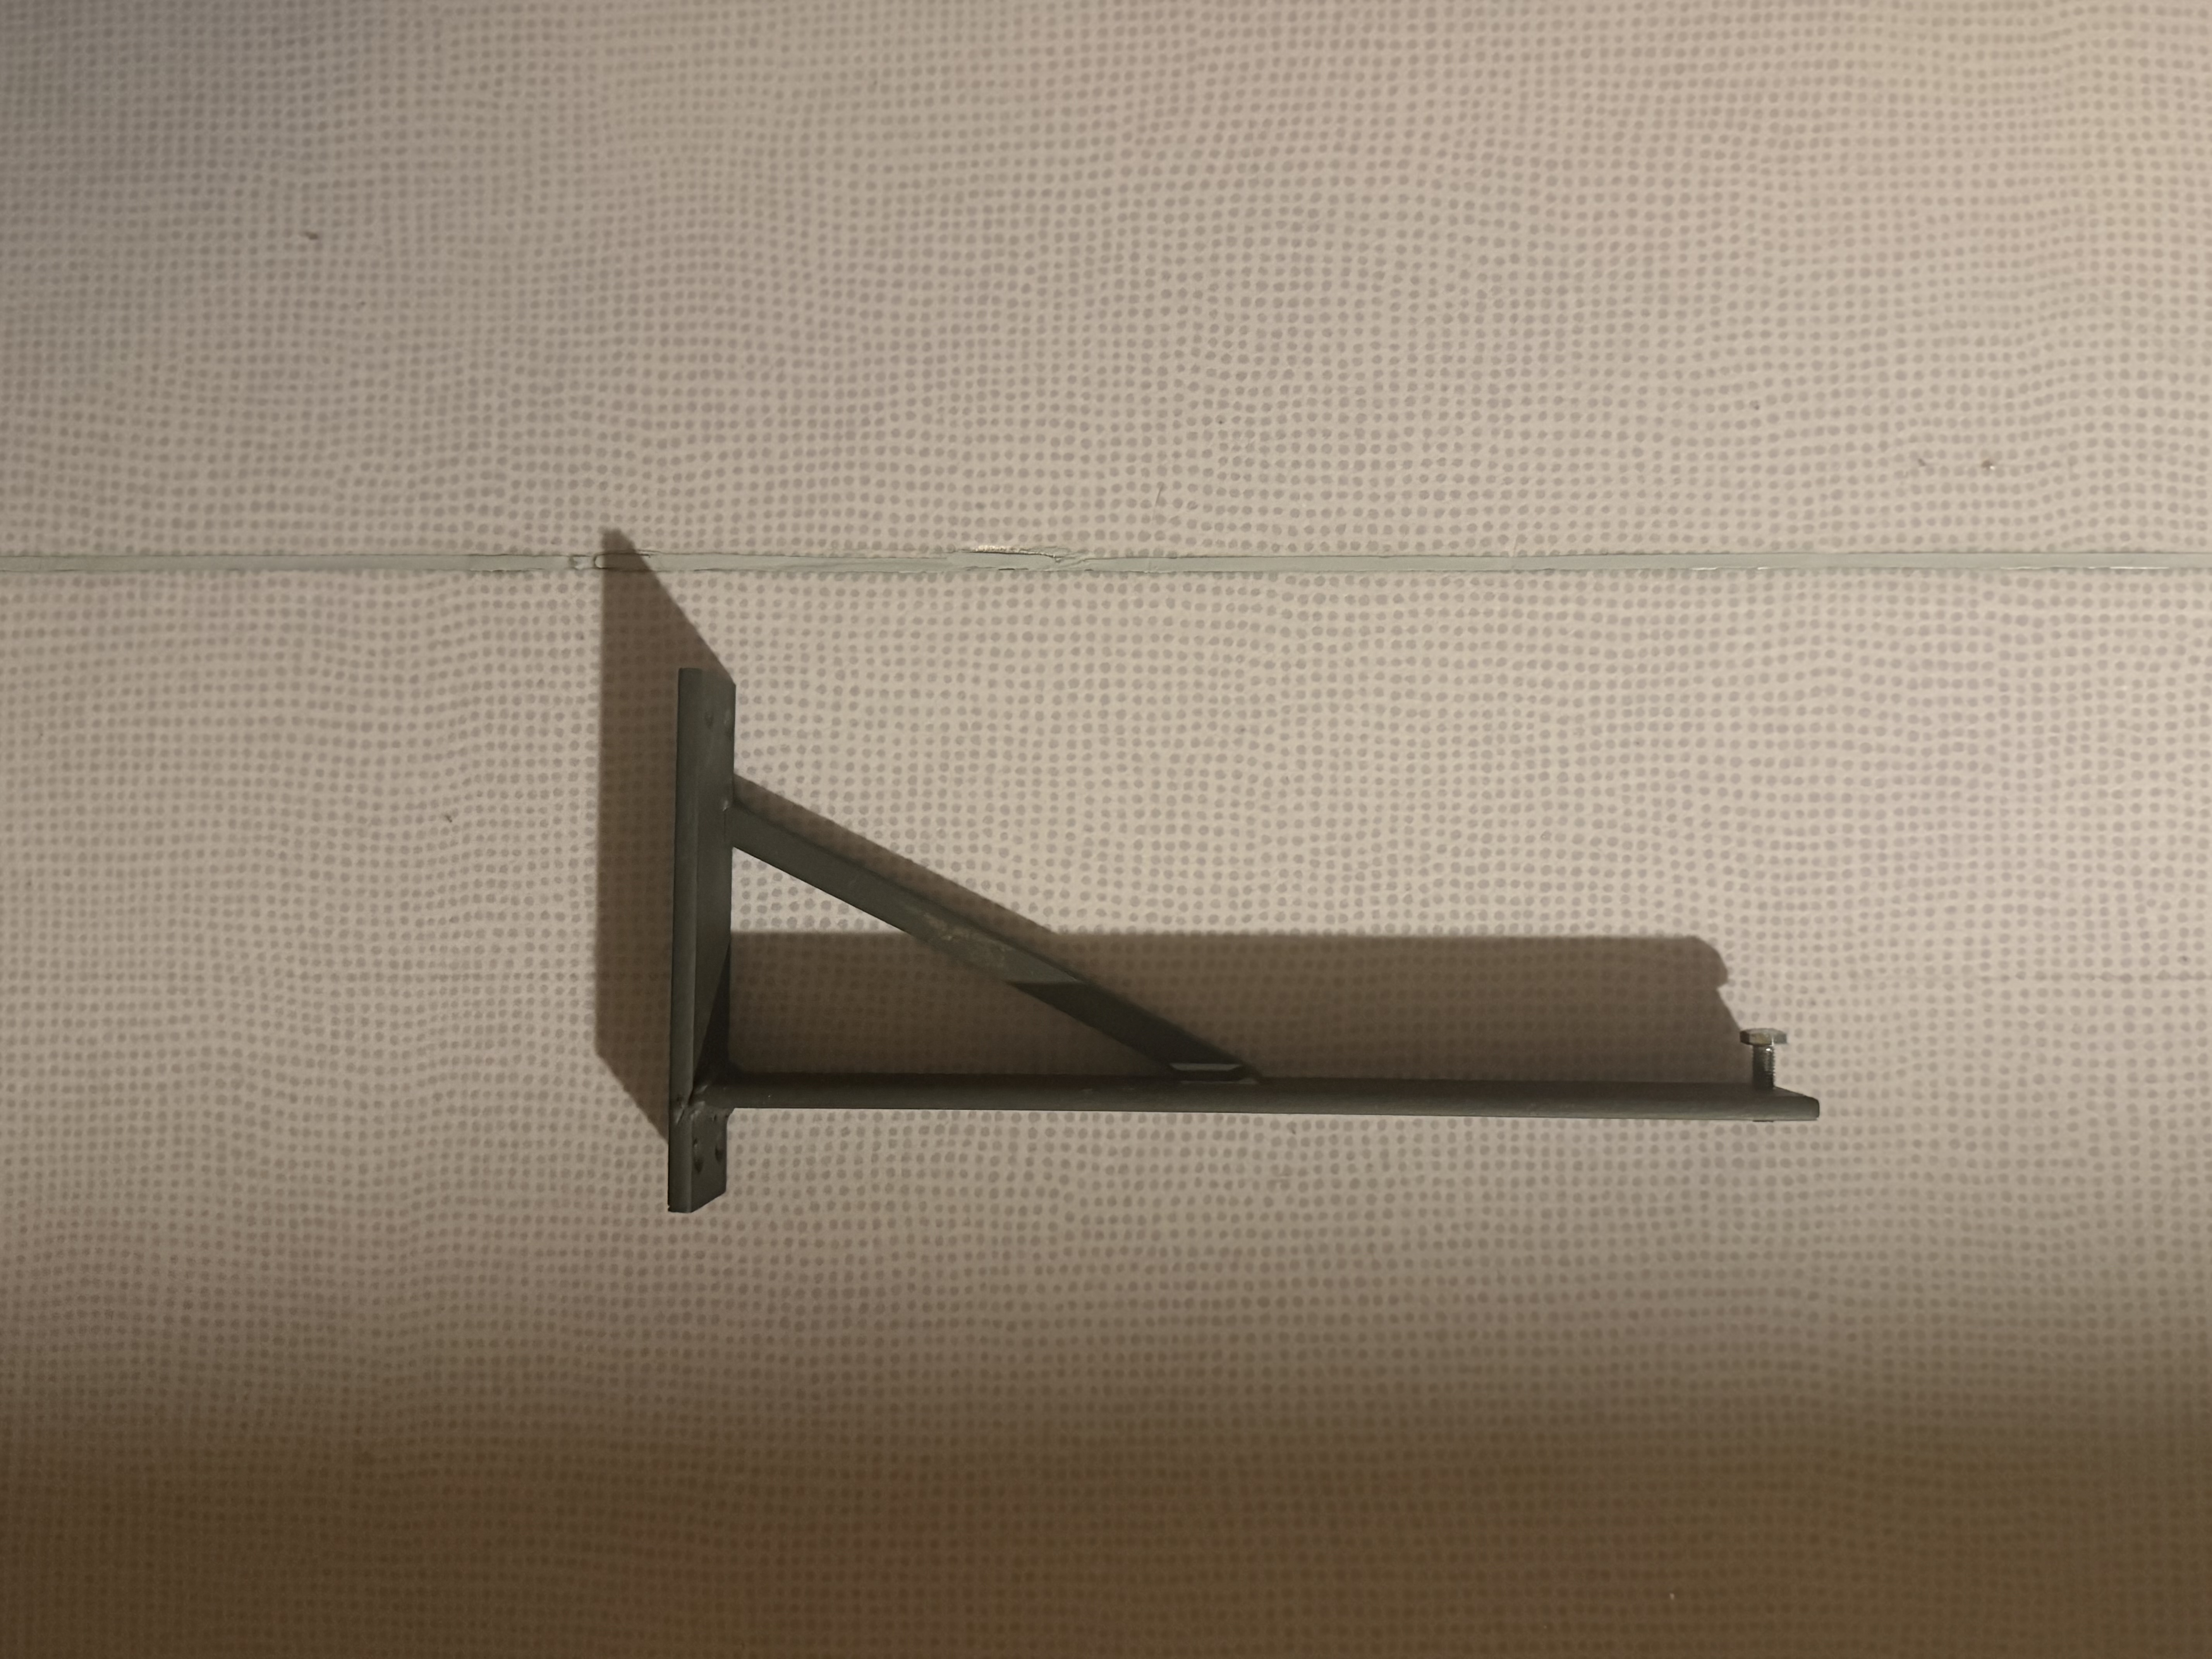
\includegraphics[width=\textwidth,height=0.4\textheight,keepaspectratio]{piece3.jpg}
    \par\vspace{2pt}{\scriptsize \textit{Pièce 3}}
    \vspace{0.2cm}
    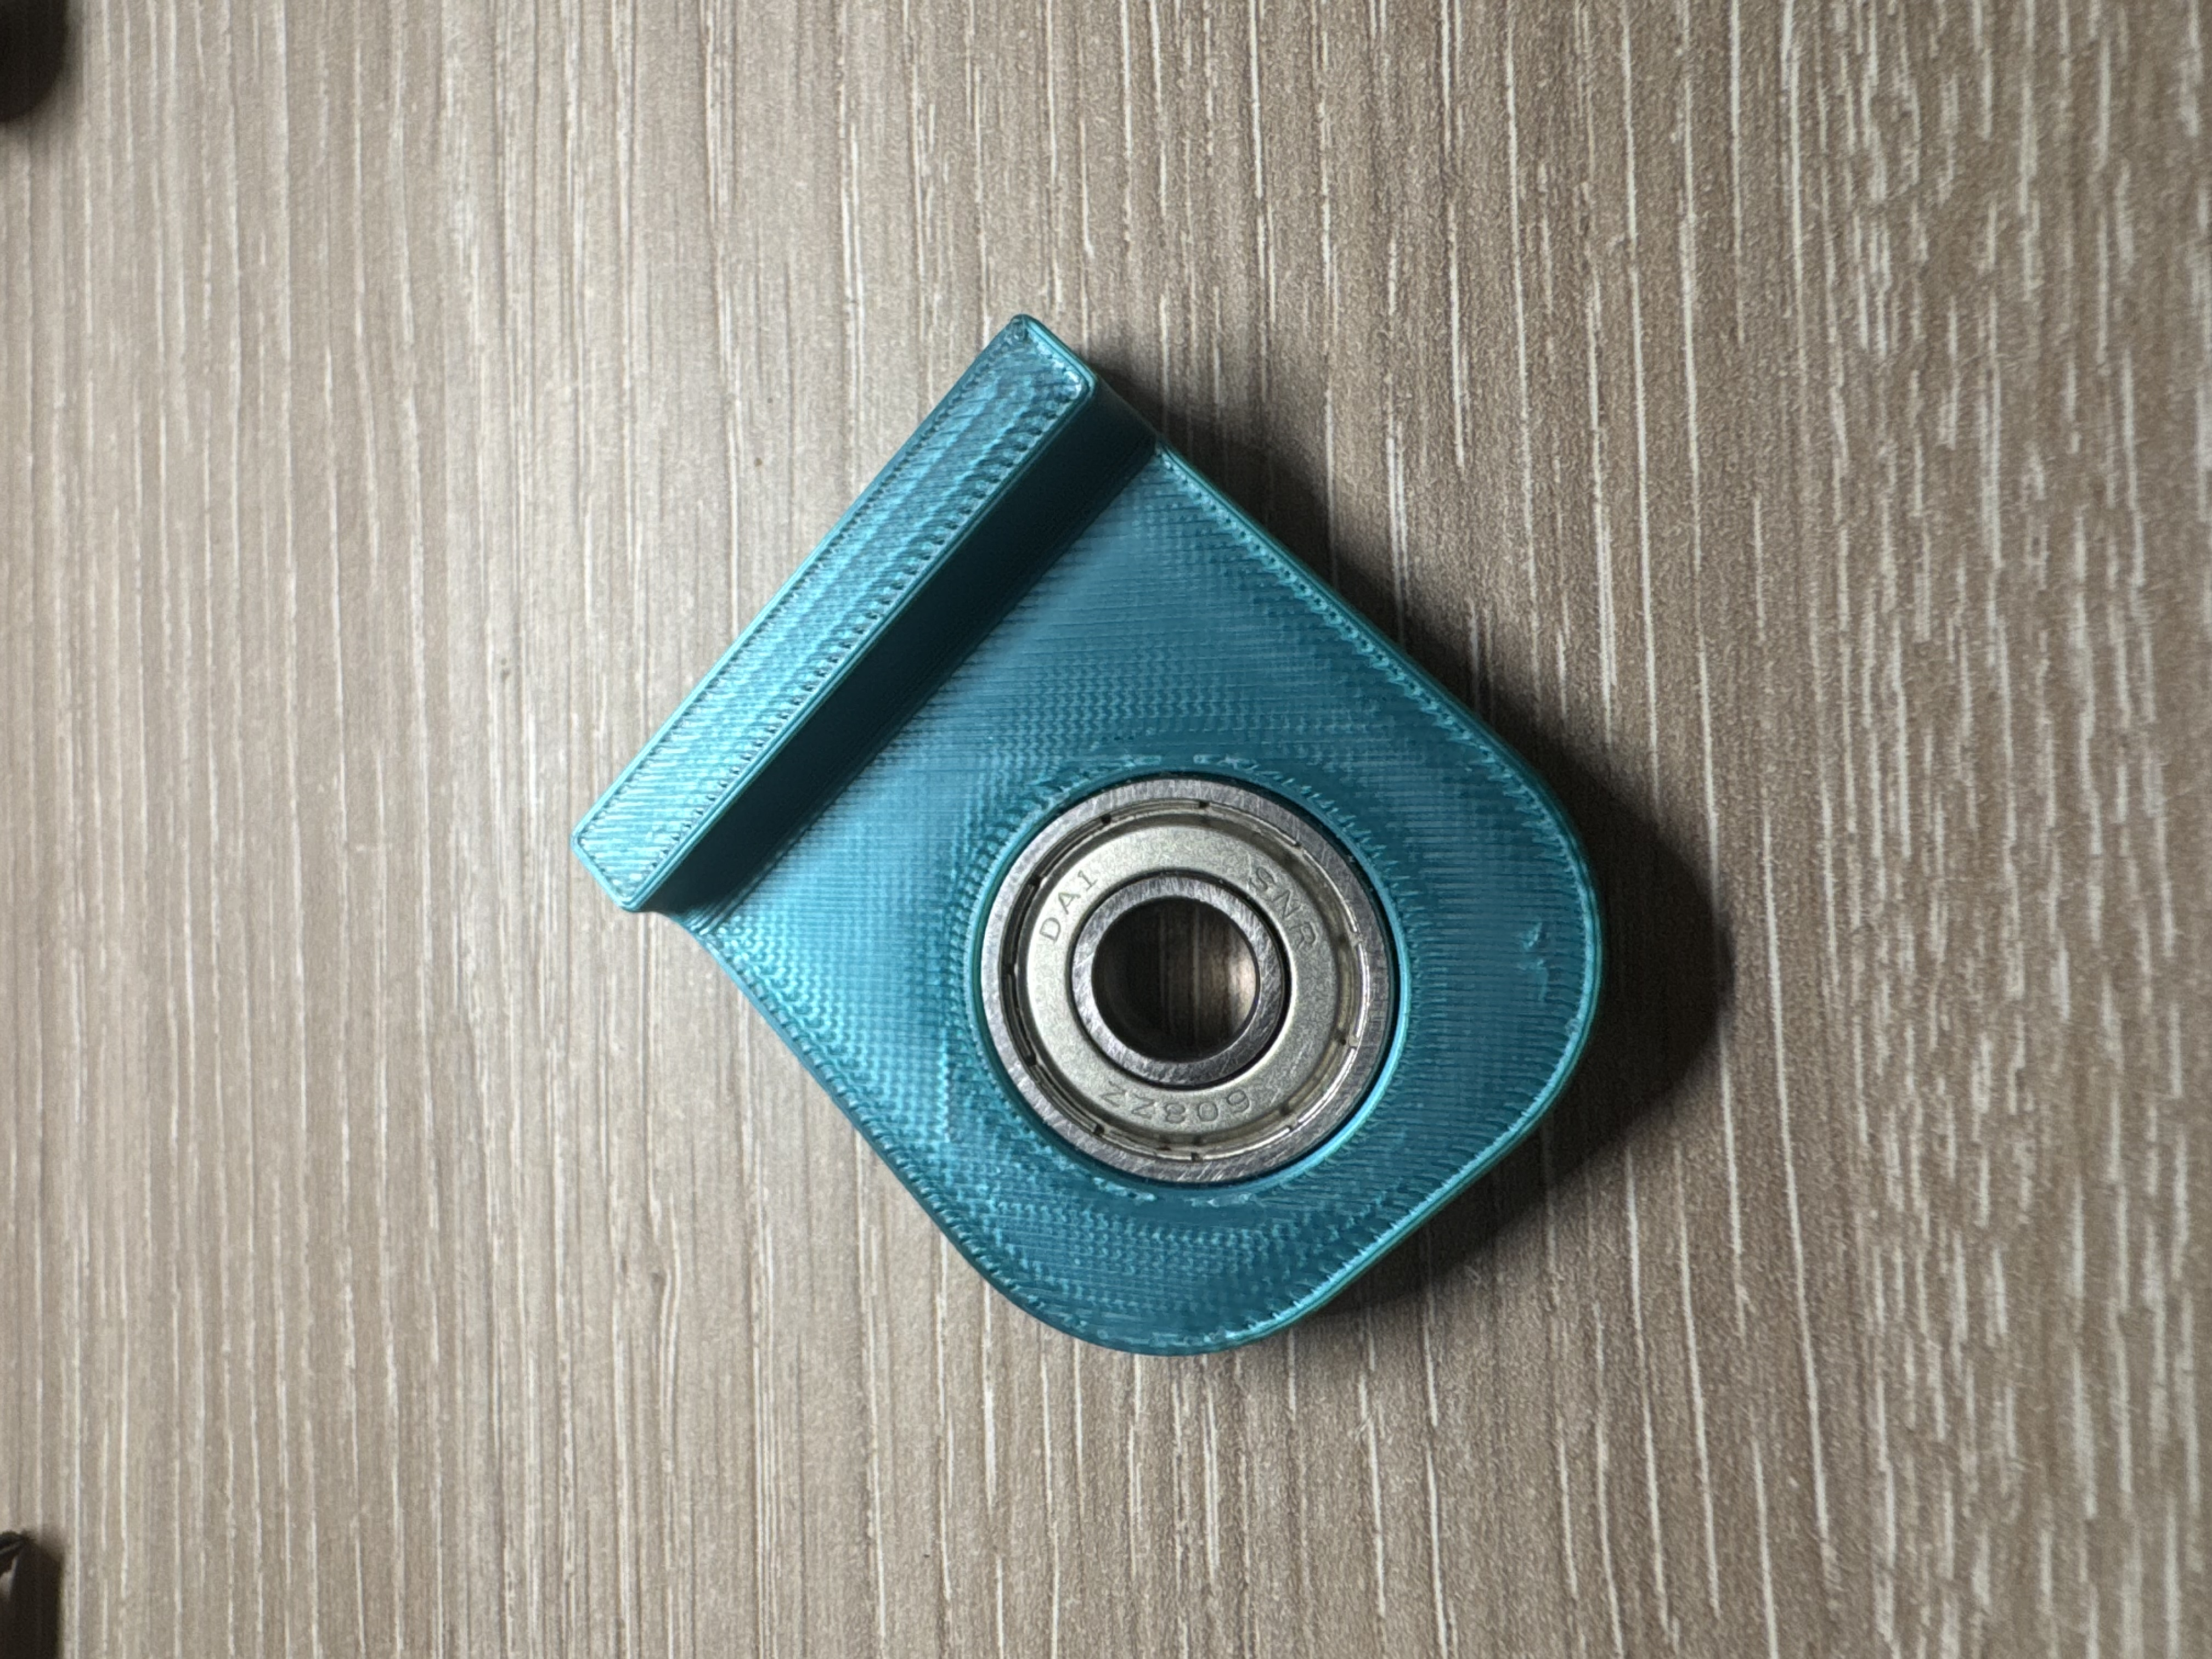
\includegraphics[width=\textwidth,height=0.4\textheight,keepaspectratio]{piece4.jpg}
    \par\vspace{2pt}{\scriptsize \textit{Pièce 4}}
  \end{columns}
\end{frame}

\begin{frame}{Annexe : Résultats Graphiques de Simulation}
  \centering
  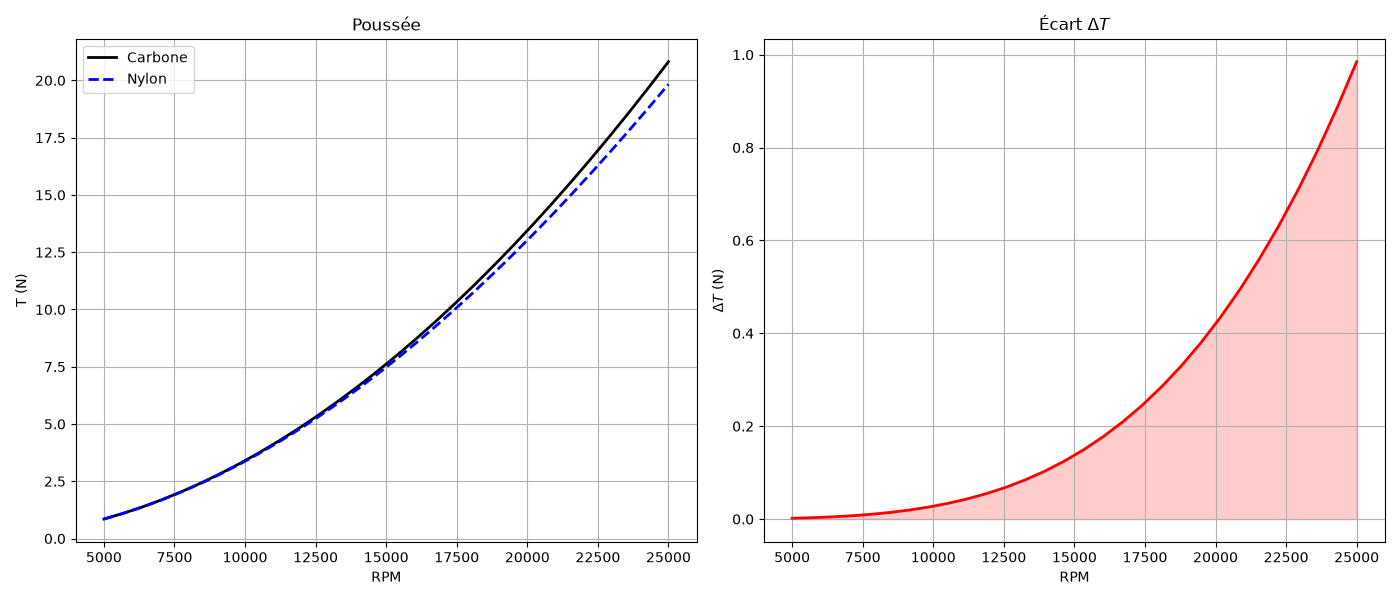
\includegraphics[width=0.75\textwidth]{resultatStrategie1.png}
\end{frame}

\begin{frame}[allowframebreaks]{Annexe : Code de Simulation Aéroélastique (\texttt{simulation1.py})}
  \lstinputlisting[language=Python]{../simulation1.py}
\end{frame}

\end{document}
